\documentclass[10pt,a4paper]{article} 
\setlength{\parindent}{0pt} 
% text formatting 
\usepackage[a4paper,left=2.4cm,right=2.4cm,top=2.4cm,bottom=2.4cm]{geometry}
% \usepackage[utf8]{inputenc} %%% 
%\usepackage{natbib}
\usepackage{hyperref}
\hypersetup{
  hidelinks,
  plainpages=false,
}
\pagestyle{empty}
\usepackage{graphicx}
% \usepackage[draft]{graphicx}
\usepackage{textcomp}
\usepackage{bbding}
\usepackage{amssymb}
\usepackage{multicol}
\setlength{\columnseprule}{1pt}
\def\columnseprulecolor{\color{grey}}
\usepackage{fancyhdr}
\setlength{\unitlength}{1in}

\usepackage{soul}
% \usepackage{xcolor}
% \newcommand{\hlone}[1]{{\sethlcolor{FFFF00}\hl{#1}}}
% \newcommand{\hltwo}[1]{{\sethlcolor{cyan}\hl{#1}}}
% \newcommand{\hlfinal}[1]{{\sethlcolor{lime}\hl{#1}}}

% table layout
\usepackage{booktabs}  % pandas tables
\usepackage{array}
\usepackage{tabularray}
\UseTblrLibrary{caption} % to make Table X bold for longtblr
\SetTblrStyle{caption-tag}{font=\bfseries}
\DefTblrTemplate{contfoot-text}{default}{}
\DefTblrTemplate{conthead-text}{default}{}
\DefTblrTemplate{capcont}{default}{}
% \SetTblrStyle{caption-text}{font=\bfseries}
\usepackage{multirow}
\usepackage{makecell}  % linebreak in table
\usepackage{longtable} % for 'long table' environment
\usepackage{rotating}
\usepackage[table]{xcolor}
% \usepackage{subcaption} %  for subfigures environments 
\usepackage{float}
\usepackage{placeins}
\usepackage{tabularx}
\usepackage{changepage}
\usepackage{lscape}
\usepackage{adjustbox}
\usepackage{afterpage}
\usepackage[labelfont=bf]{caption}
\captionsetup{justification=centering}
% \captionsetup[longtblr]{labelfont=bf}
\usepackage{subcaption}
\usepackage[acronym, nonumberlist, nopostdot, nogroupskip]{glossaries}
\usepackage{listings}
\usepackage{enumitem}
\usepackage[
	backend     = biber,
	maxbibnames = 99,
	natbib      = true,
	doi         = true,
	isbn        = false,
	url         = true,
	citestyle   = numeric,
  	sorting = none
]{biblatex}
\addbibresource{enalapril.bib}
% \usepackage{times}  %%%
\usepackage{newtxtext,newtxmath}
\usepackage{setspace}
\setstretch{1.0}

\usepackage{ragged2e}
\usepackage[T1]{fontenc} 
\usepackage{authblk}

\PassOptionsToPackage{nopatch=footnote}{microtype}
\usepackage{microtype}

% \usepackage{xr}
% \externaldocument{08_suppldata}

%svg
\usepackage{svg}
\usepackage{amsmath}
\usepackage{siunitx}

%tables
\newcolumntype{P}[1]{>{\centering\arraybackslash}p{#1}}
\newcolumntype{L}[1]{>{\raggedright\arraybackslash}p{#1}}

%for ticks in data table column "fit"
\usepackage{pifont}
\usepackage{pdflscape}
% \usepackage{color, colortbl}
% \usepackage{colortbl}
\definecolor{Lightgrey}{rgb}{0.9, 0.9, 0.9}
% \definecolor{}{HTML}{FFCC00} 
% \definecolor{Yellow}{HTML}{FFFF00}


\title{A Physiologically Based Pharmacokinetic and Pharmacodynamic (PBPK/PD) Model of Enalapril}
\author[1]{Shubhankar Palwankar}
\author[2]{Mariia Myshkina}
\author[3]{Matthias König}
\affil[1,2,3]{Institute for Biology, ITB, Humboldt-Universität zu Berlin, Philippstraße 13, 10115 Berlin, Germany}
\affil[3]{University Hospital Schleswig-Holstein, Campus Lübeck, First Department of Medicine, Ratzeburger Allee 160, 23562 Lübeck, Germany}
% \date{\today}

\begin{document}
\maketitle

\section*{Abstract}\label{sec:abstract}\justifying{}
{\color{red}
\textbf{Background/Objectives:} Dapagliflozin is an SGLT2 inhibitor prescribed for the management of type 2 diabetes mellitus. The drug lowers blood glucose levels by increasing urinary glucose excretion (UGE). Despite established efficacy, dapagliflozin demonstrates significant inter-individual variability in pharmacokinetics (PK) and pharmacodynamics (PD), with potential impact on treatment outcomes. \textbf{Methods:} To evaluate the sources of variability and to support patient stratification and model-informed individualized therapy, we developed a physiologically based pharmacokinetic/pharmacodynamic (PBPK/PD) model of dapagliflozin using curated data from 28 clinical studies. This framework integrates absorption, distribution, metabolism, excretion, and pharmacodynamics, and accounts for key determinants of variability including renal and hepatic function, and food effects. \textbf{Results:} The simulations reproduced dose-dependent pharmacokinetics with predicted Cmax and AUC values typically within 10--15\% of observed data. Renal impairment reduced UGE by 40--60\% despite modest changes in plasma exposure, while hepatic impairment produced only small shifts in PK and PD. The model also reproduced the fed-state reduction of peak concentrations, consistent with the 30--50\% decrease reported clinically. \textbf{Conclusions:} All model files, code, and curated datasets are openly available in line with FAIR standards and Open Science practices, enabling transparent and reproducible analyses and providing a mechanistic basis for individualized therapy in type 2 diabetes.
Enalapril is a medication used to treat high blood pressure and a num ber of other cardiovascular conditions. The renin-angiotensin-aldosterone system (RAAS) is the main component involved in the regulation of blood pressure in the body. One of the key steps in this process is the conversion of angiotensin I to angiotensin II by angiotensin converting enzyme(ACE). Enalapril is an ACE inhibitor and therefore helps to lower blood pressure. Pharmacokinetics is the branch of pharmacology that studies how the body absorbs, distributes, metabolizes, and eliminates drugs over time. After administration as enalapril maleate, it is absorbed in the intestine and converted by carboxylesterase 1 (CES1) in the liver to the active metabolite, enalaprilat. Enalapril and enalaprilat are eliminated from the body by renal clearance. A physiologically based pharmacokinetic (PBPK) model was developed to investigate the pharmacokinetics of enalapril and the factors influencing it. As part of the work, an extensive database of enalapril pharmacokinetics consisting of data from 49 clinical trials was established and used to parameterize and validate the computational model. The model was used to investigate the effect of renal impairment, hepatic impairment and changes in CES1 activity on the pharmacokinetics of enalapril and enalaprilat, as these three factors are known to have a major influence on the pharmacokinetics of enalapril. The model shows good agreement with a wide range of enalapril and enalaprilat data in serum, plasma and urine under different conditions (healthy, renal impairment, hepatic impairment, CES1 mutations). The model is available in SBML under a CC-BY 4.0 license with all data freely available from the PK-DB pharmacokinetics database.}

Keywords: hypertension, enalapril, pharmacokinetics, ACE inhibitor, renal impairment, hepatic impairment, CES1
\section{Introduction}\label{sec:introduction}\justifying{}
Hypertension, commonly known as high blood pressure, is a chronic cardiovascular condition in which the force of the blood against the artery walls is consistently too high. Uncontrolled hypertension significantly increases the risk of serious health problems, including heart attack, stroke and kidney disease. The renin-angiotensin-aldosterone system (RAAS) regulates blood pressure through a negative feedback mechanism where reduced renal blood flow indirectly causes the angiotensin-converting enzyme (ACE) transforming angiotensin I into angiotensin II, a potent vasoconstrictor that raises blood pressure. Angiotensin II triggers aldosterone secretion which increases sodium and water retention to maintain vascular volume and resistance. Dysfunction of the RAAS system causes hypertension, which can be managed with ACE inhibitors. These widely prescribed drugs lower blood pressure and minimize cardiovascular risk by blocking the conversion of angiotensin I to angiotensin II. Additionally, ACE inhibitors prevent the breakdown of bradykinin, a vasodilator that further reduces blood pressure and alleviates heart strain. Common examples include enalapril, lisinopril, ramipril, captopril, and benazepril, each playing a vital role in cardiovascular management~\cite{Vertes1992}.

Enalapril is an FDA-approved ACE inhibitor drug for treating hypertension. Enalapril is the esterified prodrug, usually given orally as enalapril maleate, and further hydrolysed in the liver (\textit{in vivo} de-esterification) to enalaprilat, the active metabolite involved in ACE inhibition. Enalaprilat acts as a competitive inhibitor of ACE, preventing angiotensin I from interacting with it. The resulting enzyme-inhibitor complex has a slower dissociation rate, which effectively causes ACE inhibition. 

Pharmacokinetic parameters such as maximum concentration (C\textsubscript{max}), time to peak concentration (T\textsubscript{max}), half-life (T\textsubscript{1/2}), and elimination rate (k\textsubscript{el}) inform dosing strategies that maximize efficacy while minimizing side effects. In healthy adults, enalapril has an oral bioavailability of 60\%, unaffected by food~\cite{Swanson1984}, and reaches peak plasma concentrations 1--2 hours after ingestion~\cite{Dickstein1987, MacFadyen1993, Ulm1983, VanHecken2020}. It is subsequently hydrolyzed in the liver by carboxylesterase 1 (CES1) to its only active metabolite, enalaprilat: by 4 hours post-dose, plasma enalapril levels are negligible while enalaprilat approaches its own maximum concentration, reached 3--4 hours post-biotransformation, with an independent bioavailability of approximately 40\%~\cite{Davies1984, Till1984}. Enalapril has an elimination half-life of 2--3 hours and is excreted in urine and feces, and evening administration delays its T\textsubscript{max}~\cite{Weisser1991}. Hypertension itself does not alter the pharmacokinetics of enalapril or enalaprilat~\cite{Todd1992b}, indicating that the disease being treated is not a source of pharmacokinetic variability.

Instead, this variability arises from patient- and organ-level factors, most notably age~\cite{Hockings1986, Lees1987a, MacDonald1993}, renal impairment~\cite{Fruncillo1987, Kelly1986, Lowenthal1984}, and hepatic impairment~\cite{Baba1990, Ohnishi1989}. The evidence for an age effect is mixed: Hockings et al. 1986~\cite{Hockings1986} and Lees et al. 1987~\cite{Lees1987a} found no age-related differences in pharmacokinetics or ACE inhibition between young and elderly groups, whereas MacDonald et al. 1993~\cite{MacDonald1993} reported a higher enalaprilat area under the curve (AUC) in older individuals, indicating prolonged drug exposure. This inconsistency suggests that age alone is an unreliable proxy for the underlying physiological changes that actually drive variability in enalapril pharmacokinetics, motivating a mechanistic treatment of the organ functions -- renal and hepatic -- that age-related decline, renal disease, and liver disease each affect directly.

Because pharmacokinetic exposure ultimately determines pharmacodynamic effect, the same sources of variability are expected to propagate to enalapril's action on the RAAS. For the ACE inhibitor enalapril, key pharmacodynamic parameters include blood pressure, heart rate, ACE activity, and RAAS hormone concentrations (renin, aldosterone, and angiotensins) ~\cite{Donnelly1987, Lees1987a, Ribeiro1996, Shionoiri1985}. Studies demonstrate that a 6-week daily enalapril regimen significantly reduces systolic and diastolic blood pressure, achieving near-complete ACE inhibition (\(101\%\)--\(103\%\)) ~\cite{Donnelly1990}. ACE inhibition typically peaks at 90\% within 3--5 hours post-dose and drops to 50\% at 24 hours ~\cite{Ribeiro1996}. When comparing age groups, younger and older patients show similar levels of ACE inhibition ~\cite{Lees1987a}. While older patients experience a greater absolute drop in blood pressure, this difference disappears when normalized as a percentage, meaning the larger decrease is simply due to their higher baseline blood pressure~\cite{Lees1987a}.

Since enalapril and enalaprilat are eliminated almost exclusively via the kidneys, renal dysfunction directly alters their pharmacokinetics: progressive renal impairment reduces urinary elimination of enalapril, raising peak serum enalapril levels and increasing its conversion to enalaprilat~\cite{Fruncillo1987}, so that patients with renal failure show higher serum enalaprilat concentrations, longer T\textsubscript{max}, and lower excretion rates for both the parent drug and its metabolite~\cite{Kelly1986, Lowenthal1985}. Because enalapril additionally depends on hepatic CES1-mediated conversion to become active, liver dysfunction represents a second, independent route by which organ function shapes exposure -- though here the evidence is less consistent. Ohnishi et al.~\cite{Ohnishi1989} found that cirrhotic patients had higher enalapril C\textsubscript{max} and AUC alongside lower urinary excretion, indicating impaired hepatic processing, whereas Baba et al. 1990~\cite{Baba1990} reported no significant differences in C\textsubscript{max}, T\textsubscript{max}, or ACE inhibition between cirrhotic and healthy subjects. Renal and hepatic function thus each independently, and potentially jointly, determine enalapril exposure, motivating a model that can separate and combine their effects rather than treating impairment as a single covariate.

Genetic variation in CES1 provides a third, molecularly defined source of variability. The loss-of-function G143E variant severely impairs enalapril metabolism: carriers show an approximately 20--27.5\% reduction in enalaprilat AUC, lower peak concentrations, and a roughly 30\% delay in T\textsubscript{max}~\cite{Her2021, Tarkiainen2015}, with a correspondingly diminished therapeutic effect -- a negligible systolic blood pressure drop (-1.0 mmHg) compared to 14.6 mmHg in wild-type patients~\cite{Her2021}. Stage et al. 2017~\cite{Stage2017} evaluated additional complex variants, including copy-number variations (3-copy and 4-copy) and structural changes (CES1A2, CES1A1c); while several reduced enzymatic activity or prolonged T\textsubscript{1/2}, median enalaprilat AUC across these variants did not differ significantly from wild type. CES1 genotype therefore modulates enalapril pharmacokinetics through the same hepatic conversion step affected by cirrhosis, but via a distinct, genetically defined mechanism that a purely organ-function-based model cannot capture on its own.

With this study, we aim to develop a reproducible, openly available PBPK/PD model of enalapril, built from published data in healthy subjects and patients with hypertension, renal impairment, and hepatic impairment. This allows comparative analysis across health states to understand how hepato-renal function and CES1 activity affect enalapril's distribution, metabolism, and excretion. Because enalapril's effects vary with patient characteristics, organ impairment, and CES1 genetic variation, the model provides a framework for predicting drug behavior across these conditions -- supporting more personalized dosing strategies and filling gaps in current mechanistic understanding.
\section{Methods}\label{sec:methods}\justifying{}
The methods used in this work consisted of a systematic literature search for enalapril (Sec.~\ref{sec:methods_lit_search_data_curate}), followed by data curation (Sec.~\ref{sec:methods_data_curation}), simulation of data for each study (Sec. ~\ref{sec:methods_simulations}), parameter optimisation by fitting simulated data to reference data (Sec.~\ref{sec:methods_fitting}), parameter scans for renal function, liver function and CES1 activity (Sec.~\ref{sec:methods_scans}) and calculation of pharmacokinetic parameters (Sec.~\ref{sec:methods_pk_parameters}).

\subsection{Systematic literature research and Data curation}
\label{sec:methods_lit_search_data_curate} 
Data on the pharmacokinetics and pharmacodynamics of enalapril under different conditions was collected using a systematic literature search. \href{https://pubmed.ncbi.nlm.nih.gov/}{PubMed} and \href{https://www.pkpdai.com/}{PKPDAI}~\cite{GonzalezHernandez2021} were searched using the keywords \texttt{enalapril AND pharmacokinetics OR pharmacodynamics} and keyword \texttt{enalapril} respectively, to retrieve an initial corpus of literature on the pharmacokinetics of enalapril. Articles on clinical trials of enalapril were selected based on pre-specified inclusion criteria. In addition to healthy subjects, trials in patients with hypertension, renal, cardiac and hepatic impairment were included. Studies in paediatric patients and animal studies were excluded as also were studies with insufficient data. Fig.~\ref{fig:ena_lit_search} provides an overview of the literature review process. In addition, the literature was searched for \textit{in vitro} studies to determine kinetic parameters and enzyme kinetic information. Data were systematically curated to capture patient demographics, organ impairment states, and trial intervention parameters such as dose, route, and timing of enalapril administration. Additionally, time course concentrations of enalapril and its metabolite enalaprilat in serum, plasma, and urine were recorded alongside key pharmacokinetic parameters (C\textsubscript{max}, T\textsubscript{max}, T\textsubscript{1/2}) and pharmacodynamic outcomes like blood pressure, heart rate, and renin-angiotensin-aldosterone markers. The articles were screened for patient information such as age, sex, specific diseases, drugs and genotypes, enalapril dosing protocol and enalapril pharmacokinetic profiles. These data were then curated using standard protocols for pharmacokinetic information~\cite{Grzegorzewski2021}. Data from figures were digitised using WebPlotDigitizer~\cite{Rohatgi2024}. Data from tables and textual descriptions were also curated in a specific format as described in~\cite{Grzegorzewski2021}. Data thus collected from the selected literature was curated and uploaded to the open pharmacokinetics database \href{https://alpha.pk-db.com/}{PK-DB}~\cite{Grzegorzewski2021} with an overview of the curated studies in Tab.
% ~\ref{tab:study_table}.

\subsection{Model}
The PBPK and tissue models were developed in the Systems Biology Markup Language (SBML)~\citep{Hucka2019, Keating2020}. Software such as sbmlutils~\citep{Konig2023} and cy3sbml~\citep{Konig2012} were used for the programmatic manipulation and visualisation of the models. The models are ordinary differential equation (ODE) models solved numerically using sbmlsim~\citep{Konig2021} based on the high performance SBML simulator libroadrunner~\citep{Somogyi2015, Welsh2023}. The model is made available in SBML under a CC-BY 4.0 licence from \url{https://github.com/matthiaskoenig/enalapril-model} with model equations available from the repository. The version of the model used in this thesis is \href{https://zenodo.org/doi/10.5281/zenodo.11067564}{0.9.5}~\cite{enalapril-model-v0.9.5}.
\begin{figure}[!ht]
    \centering
    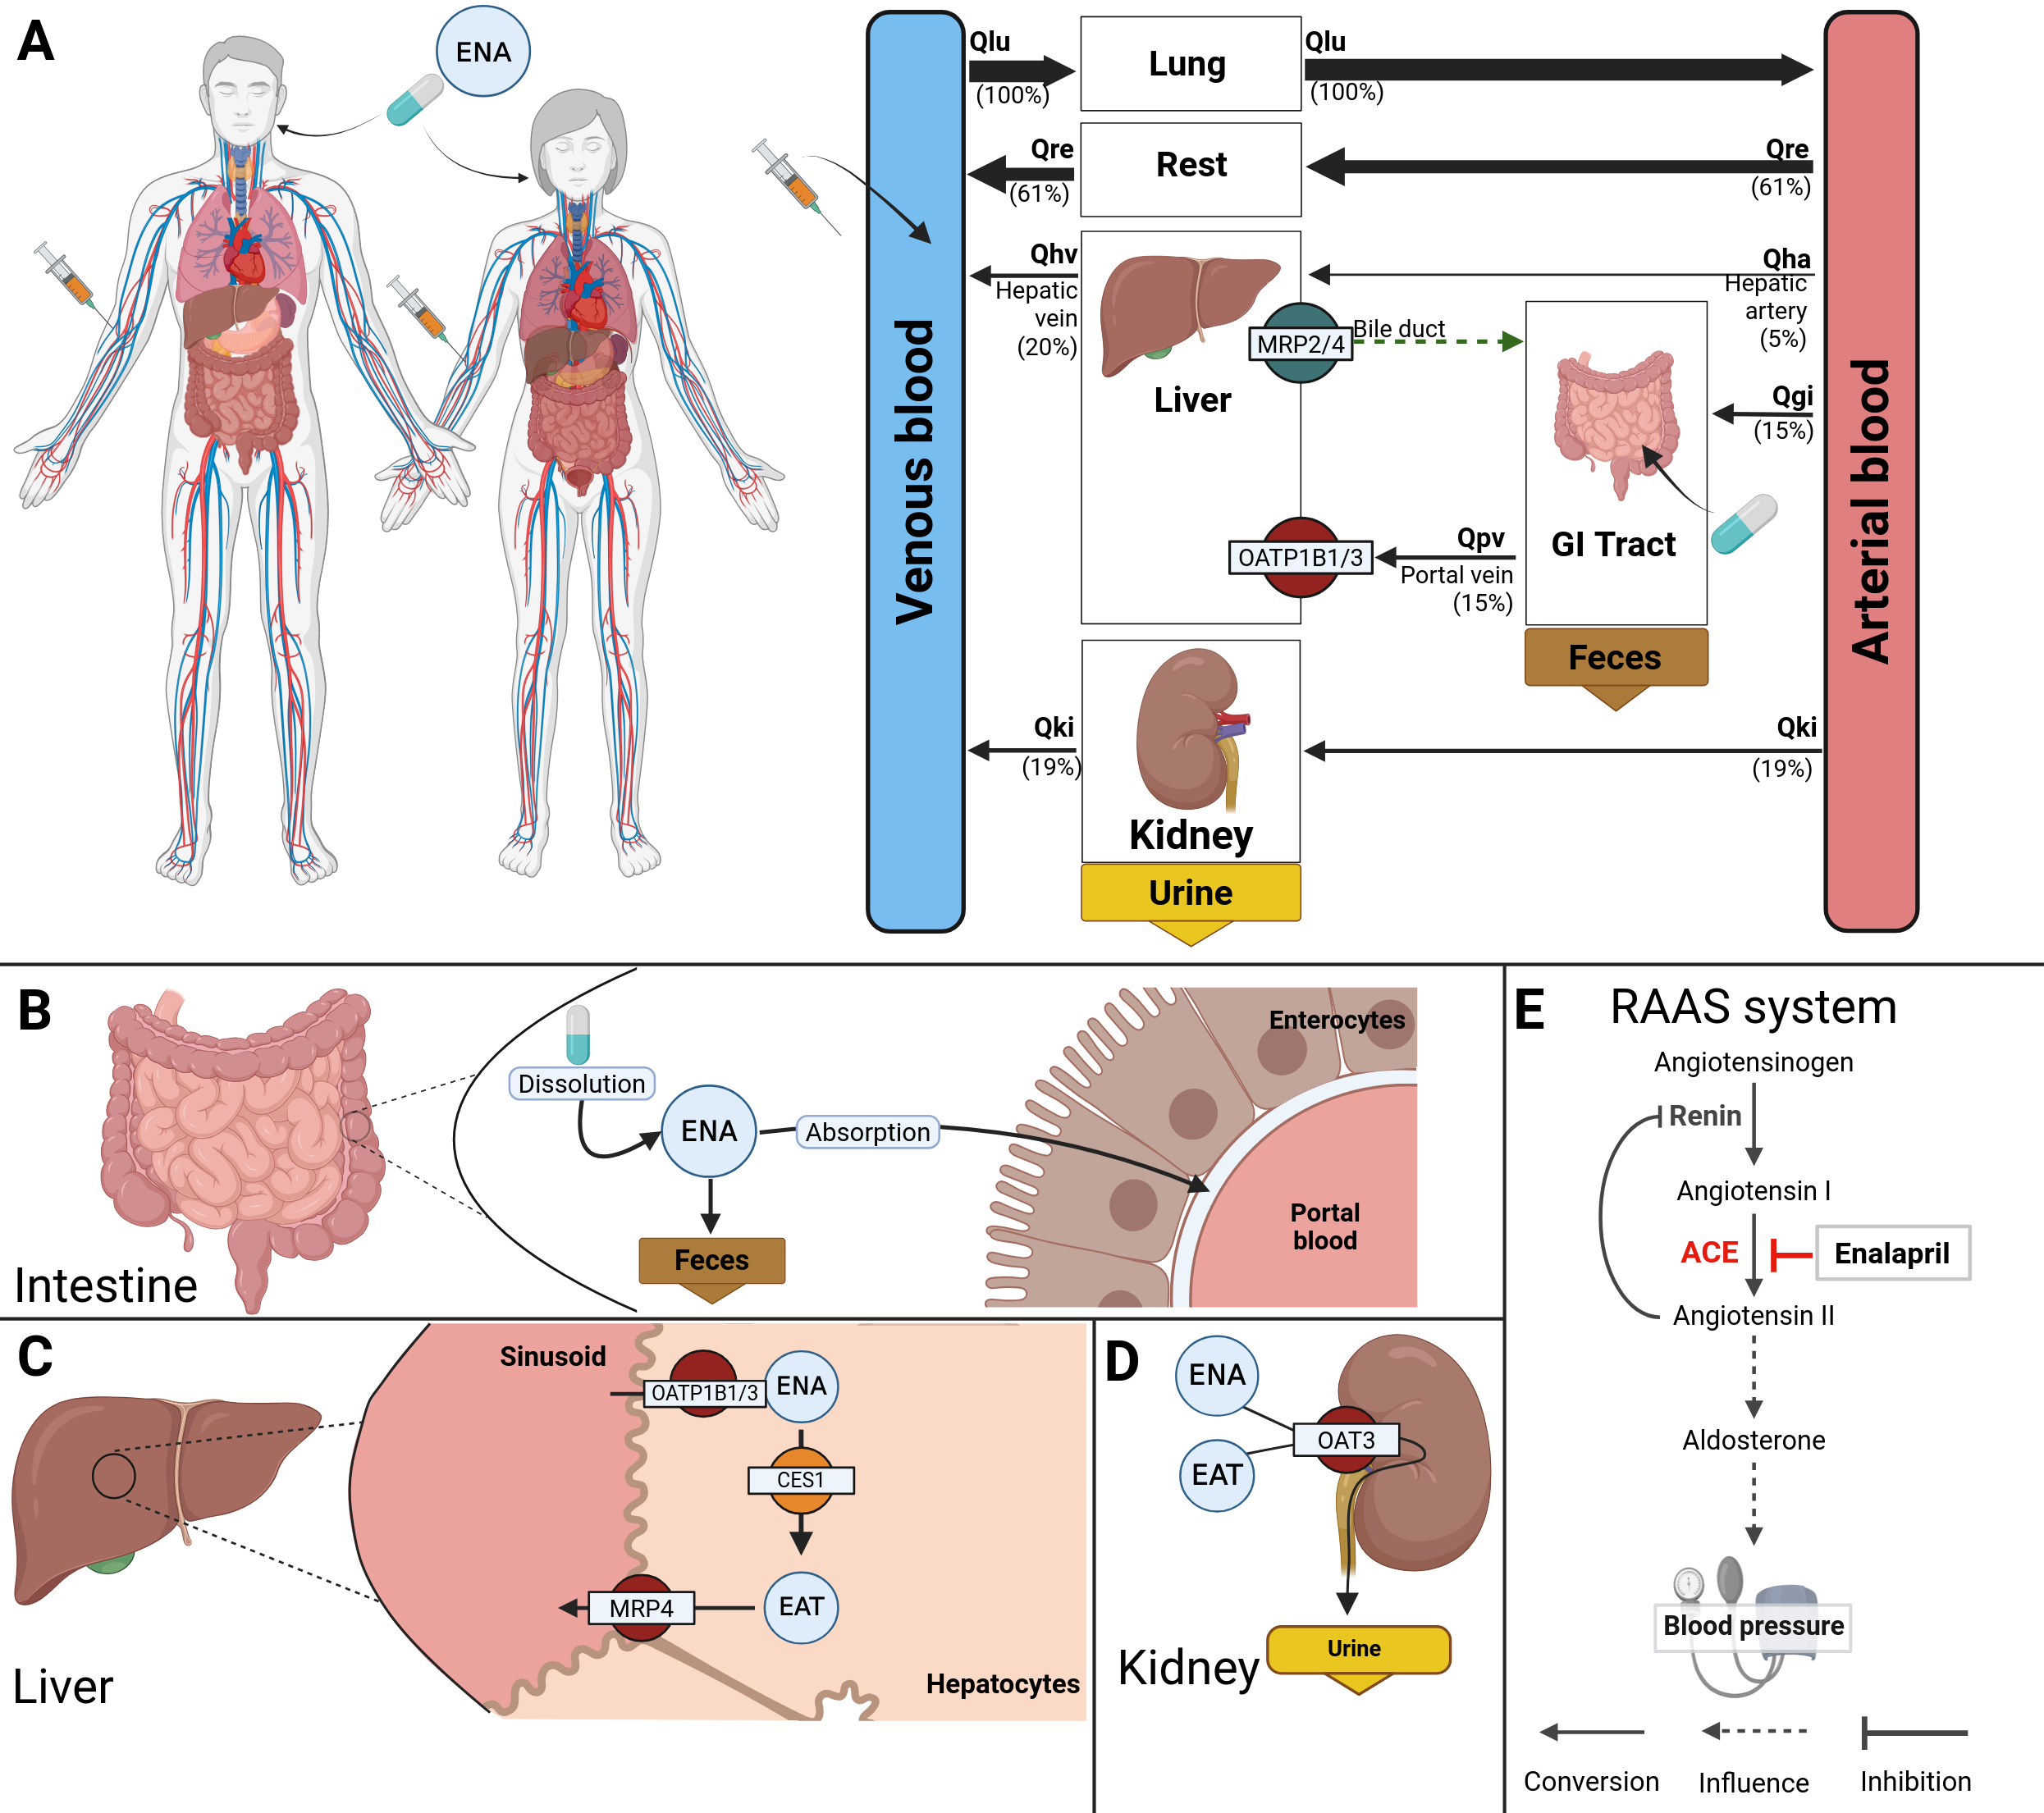
\includegraphics[width=0.99\linewidth]{figures/enalapril_model.png}
    \caption[PBPK model of enalapril]{\textbf{Overview of the physiologically-based model of enalapril.}} \textbf{(A)}~Whole body model showing cardio-pulomonary circulation via the blood. \textbf{(B)}~Intestine model showing dissolution and absorption of enalapril by enterocytes. \textbf{(C)}~Liver model with the uptake of enalapril by hepatocytes and its conversion to enalaprilat. \textbf{(D)}~Kidney model showing transport of enalapril and enalaprilat into the kidney and their subsequent excretion via urine. \textbf{(E)}~Schematic of the renin-angiotensin-aldosterone system (RAAS)  and the interfering/inhibitory role of enalapril
    \label{fig:enalapril_model}
\end{figure}

The PBPK model developed consists of a whole-body model linking different organs via the systemic circulation (Fig.~\ref{fig:enalapril_model}). The PBPK model follows a hierarchical structure, with the whole-body model linking sub-models for the intestine, kidney and liver.The model describes the metabolic and biochemical pathways in the tissue consisting of the transport of enalapril through the intestine, liver and kidney. Transport processes and biochemical reactions were modelled using reversible and irreversible Michaelis-Menten equations.

Liver impairment was modeled by scaling liver function with \texttt{f\_cirrhosis} from 0.0 (no cirrhosis) to 0.95 (critical cirrhosis), based on an indocyanine green model~\cite{Koller2021, Koller2021a} mapping CPT classes A, B, and C to parameter values of 0.40, 0.70, and 0.81, respectively. The Child-Turcotte-Pugh (CTP) score estimates mortality risk in cirrhotic patients using criteria originally outlined by Child and Turcotte~\cite{Child1964} and later modified by Pugh~\cite{Pugh1973}. Mechanistically, cirrhosis is represented by reduced functional liver volume alongside portosystemic blood shunting, both decreasing effective liver blood flow. 
Renal impairment was modeled as a progressive functional decline by scaling all renal processes with \texttt{f\_renal\_function} (1.0 = normal, 0.0 = none), applying KDIGO-based cut-offs~\cite{Stevens2024} for mild (0.69), moderate (0.32), and severe (0.19) stages~\cite{Mallol2023}.
Cardiac impairment was simulated by reducing total blood flow by 30\% using \texttt{f\_cardiac\_output} = 0.70.
Variations in CES1 activity were modeled by scaling the metabolic rate via \texttt{f\_ces1} (wild type = 1.0, $>1.0$ = increased, $<1.0$ = reduced). Modeled alleles included wild type (1.0), G143E (0.1), active allele (1.2), and CES1A1C (1.0), with overall function calculated as the average of both alleles (e.g., WT/G143E = 0.55).

% \subsection{Model Assumptions}
% \label{sec:methods_assumptions}

\subsection{Parameter optimization}
\label{sec:methods_fitting}
Parameter fitting was used to minimise the distance between experimental data and model predictions by optimising a subset of ten parameters of the model. For this purpose, a subset of curated time curves from healthy and hypertensive subjects after single dose application was used, as listed in Tab.
% ~\ref{tab:study_table}
Parameters were optimised in a multistep process based on the route of administration. First, parameters relevant to intravenous enalaprilat were optimised using the subset of intravenous data. Next, parameters for oral enalapril were optimised using a subset of the oral enalapril data. Finally, metabolic conversion and liver transport parameters were optimised. This strategy allowed the parameters of enalaprilat and enalapril to be determined separately with subsequent optimisation of the coupling step.

The cost function, which depends on the parameter $\vec{p}$, minimised the sum of the quadratic weighted residuals $r_{i,k}$ for all time courses $k$ and data points $i$. Time courses were weighted by the number of participants in each study $n_k$ and individual time points with the standard deviation $\sigma_{i,k}$ associated with the measurement, resulting in weights $w_{i,k} = n_k/\sigma_{i,k}$.

\begin{equation*}
   F(\vec{p})= 0.5 \sum_{i,k} (w_{i,k} \cdot r_{i,k}(\vec{p}))^2
\end{equation*}

Multiple optimisation runs (n=100) were performed with different initial parameters based on a local optimiser, with the optimal parameters used in the final model. The fitted parameters are shown in Tab.~\ref{tab:Parameter_Fitting}. For validation, all data after multiple applications, disease states, CES1 activity other than wild-type were used.

\subsection{Simulations}
\label{sec:methods_simulations}
For all curated clinical trials (Tab.~\ref{tab:study_table}), \textit{in silico} simulation experiments were created. For the simulations, the parameters corresponding to the the genetic variants (\texttt{f\_ces1}), pathophysiology (\texttt{f\_renal\_function}, \texttt{f\_cirrhos
is}, \texttt{f\_cardiac\_output}),  and the dosing (\texttt{PODOSE\_ena}, \texttt{IVDOSE\_ena}, \texttt{PODOSE\_eat}, \texttt{IVDOSE\_eat}) were modified according to the study. In the case of multiple dosing, the appropriate doses were given at the specified times. The model was then used to simulate the time courses of enalapril and enalaprilat in plasma and urine, and clinical data were compared with the model predictions.

\subsection{Parameter scans}
\label{sec:methods_scans}
Parameter scans were performed for a single oral dose of enalapril of 20~mg across three main cases: liver impairment, kidney impairment and CES1 gene activity. The parameters were scanned in the following ranges: \texttt{f\_cirrhosis} in linspace (0, 0.9, num=19) with normal liver function corresponding to 0.0; \texttt{f\_renal\_function} in logspace (-1, 1, num=19) with normal kidney function corresponding to 1.0; \texttt{f\_ces1} in logspace (-1, 1, num=19) with normal CES1 function corresponding to 1.0. 

\subsection{Pharmacokinetic and pharmacodynamic parameters}
\label{sec:methods_pkpd_parameters}
Pharmacokinetic parameters of enalapril and enalaprilat were calculated from plasma concentration time curves and urinary excretion using standard non-compartmental methods. The elimination rate $k\textsubscript{el}$[1/min] was calculated by linear regression in logarithmic space in the decay phase. The area under the curve AUC [mmole$\cdot$min/L] was calculated using the trapezoidal rule and extrapolated to infinity by linear interpolation. Apparent clearance $Cl$ [ml/min] was calculated as $Cl/F = k_\mathrm{el} \cdot V_\mathrm{d}$ with apparent volume of distribution $V_\mathrm{d}/F = D/(AUC_\infty \cdot k_{el})$. $D$ is the applied dose of enalapril maleate.
***pharmacodynamic parameters***
\section{Results}\label{sec:Results}\justifying{}
\subsection{Database of enalapril pharmacokinetics}
A comprehensive literature search on the PKPD of enalapril was performed in the literature databases~\href{https://www.pkpdai.com/}{PKPDAI}~\cite{GonzalezHernandez2021} and ~\href{https://pubmed.ncbi.nlm.nih.gov/}{PubMed}. From over 600 trials assessed, 91 were prioritised according to the following criteria: (1) the study had to be conducted in humans; (2) the study had to be conducted in adult subjects; (3) the study had to be conducted \textit{in vivo}; (4) the study had to report time-course data on plasma or serum and urine concentrations of enalapril and/or its metabolite enalaprilat. Particular attention was paid to studies in subjects with hypertension and renal, hepatic and cardiac impairment. Based on these criteria, 49 studies were selected for data curation, which formed the database for the development and evaluation of the PBPK model. 
% Data was curated from Arafat et al. 2005~\cite{Arafat2005}, Baba et al. 1990~\cite{Baba1990}, Biollaz et al 1982~\cite{Biollaz1982}, Dayyih et al. 2017~\cite{Dayyih2017}, Dickstein et al. 1987~\cite{Dickstein1987}, Donnelly et al. 1990~\cite{Donnelly1990}, Fruncillo et al. 1987~\cite{Fruncillo1987}, Ghosh et al. 2012~\cite{Ghosh2012}, Gu et al. 2004~\cite{Gu2004}, He et al. 2014~\cite{He2014}, Her et al. 2021~\cite{Her2021}, Hockings et al. 1986~\cite{Hockings1986}, Howes et al. 1991~\cite{Howes1991}, Ishizaki et al. 1988~\cite{Ishizaki1988}, Johnston et al. 1992~\cite{Johnston1992}, Kelly et al. 1986~\cite{Kelly1986}, Lee et al. 2003~\cite{Lee2003}, Lees et al. 1987~\cite{Lees1987a}, Lowenthal et al. 1985~\cite{Lowenthal1985}, Lu et al. 2009~\cite{Lu2009}, MacDonald et al. 1993~\cite{MacDonald1993}, Marzo et al. 2002~\cite{Marzo2002}, Matalka et al. 2002~\cite{Matalka2002}, Moffett et al. 2014~\cite{Moffett2014}, Mujais et al. 1992~\cite{Mujais1992}, Najib et al. 2003~\cite{Najib2003a}, Niopas et al. 2004~\cite{Niopas2004}, Oguchi et al. 1993~\cite{Oguchi1993}, Ohnishi et al. 1989~\cite{Ohnishi1989}, Portoles et al. 2004~\cite{Portoles2004}, Ribeiro et al. 1996~\cite{Ribeiro1996}, Schwartz et al. 1985~\cite{Schwartz1985}, Shionoiri et al. 1985~\cite{Shionoiri1985}, Shioya et al. 1992~\cite{Shioya1992}, Stage et al. 2017~\cite{Stage2017}, Sunaga et al. 1995~\cite{Sunaga1995}, Swanson et al. 1984~\cite{Swanson1984}, Tarkiainen et al. 2015~\cite{Tarkiainen2015}, Thongnopnua et al. 2005~\cite{Thongnopnua2005}, Till et al. 1984~\cite{Till1984}, Tsuruoka et al. 2007~\cite{Tsuruoka2007}, Ulm et al. 1982~\cite{Ulm1982}, VanHecken et al. 2020~\cite{VanHecken2020}, Wade et al. 1992~\cite{Wade1992}, Weisser et al. 1991~\cite{Weisser1991}, Weisser et al. 1992~\cite{Weisser1992}, and Witte et al. 1993~\cite{Witte1993}.
Tab~\ref{tab:study_table}. provides an overview of the curated studies and key information such as number of subjects, dosing protocol, route of administration, diseases, physiological impairments and genetic variants. All data have been uploaded to the pharmacokinetics database \href{https://pk-db.com}{PK-DB}~\cite{Grzegorzewski2021} and are freely accessible via the PK-DB study identifiers.
\begin{table}[h!]
\centering
\caption[Curated clinical studies]{\textbf{Overview of curated clinical studies.} po: oral, iv: intravenous}
\vspace{0.1cm}
{\fontsize{7}{9}\selectfont
    
\begin{tabular}{L{0.12\textwidth} L{0.068\textwidth} L{0.057\textwidth} L{0.035\textwidth} L{0.05\textwidth} L{0.035\textwidth} L{0.05\textwidth} L{0.035\textwidth} L{0.035\textwidth} L{0.035\textwidth} L{0.035\textwidth} L{0.035\textwidth} L{0.05\textwidth}}
\textbf{Study} & \textbf{PK-DB} & \textbf{PMID} & \textbf{route} & \textbf{substance} & \textbf{dosing} & \textbf{dose [mg]} & \textbf{healthy} & \textbf{hyper\-tension} & \textbf{renal impairment} & \textbf{hepatic impairment} & \textbf{cardiac impairment} & \textbf{CES1} \\

\hline

\rowcolor{Lightgrey}
Arafat2005 \cite{Arafat2005} & \href{https://identifiers.org/pkdb:PKDB00741}{PKDB00741} & \href{https://pubmed.ncbi.nlm.nih.gov/15985045/}{15985045} & po & enamal & single & 10 & \checkmark &  &  &  &  & \\
Baba1990 \cite{Baba1990} & \href{https://identifiers.org/pkdb:PKDB00740}{PKDB00740} & \href{https://pubmed.ncbi.nlm.nih.gov/2165799/}{2165799} & po & enamal & single & 10 & \checkmark &  &  & \checkmark &  & \\
\rowcolor{Lightgrey}
Biollaz1982 \cite{Biollaz1982} & \href{https://identifiers.org/pkdb:PKDB00768}{PKDB00768} & \href{https://pubmed.ncbi.nlm.nih.gov/6289859/}{6289859} & po & enamal & single & 10 & \checkmark &  &  &  &  & \\
Dayyih2017 \cite{Dayyih2017} & \href{https://identifiers.org/pkdb:PKDB00769}{PKDB00769} & \href{https://pubmed.ncbi.nlm.nih.gov/28894622/}{28894622} & po & enamal & single & 20 & \checkmark &  &  &  &  & \\
\rowcolor{Lightgrey}
Dickstein1987 \cite{Dickstein1987} & \href{https://identifiers.org/pkdb:PKDB00770}{PKDB00770} & \href{https://pubmed.ncbi.nlm.nih.gov/3034316/}{3034316} & po, iv & enamal, eat & single & 5, 10 & \checkmark &  &  &  & \checkmark & \\
Donnelly1990 \cite{Donnelly1990} & \href{https://identifiers.org/pkdb:PKDB00771}{PKDB00771} & \href{https://pubmed.ncbi.nlm.nih.gov/2154407/}{2154407} & po & enamal & single, multi & 20 &  & \checkmark &  &  &  & \\
\rowcolor{Lightgrey}
Fruncillo1987 \cite{Fruncillo1987} & \href{https://identifiers.org/pkdb:PKDB00773}{PKDB00773} & \href{https://pubmed.ncbi.nlm.nih.gov/3037160/}{3037160} & po & enamal & single, multi & 5 &  & \checkmark & \checkmark &  &  & \\
Ghosh2012 \cite{Ghosh2012} & \href{https://identifiers.org/pkdb:PKDB00746}{PKDB00746} & \href{https://pubmed.ncbi.nlm.nih.gov/21341376/}{21341376} & po & enamal & single & 20 & \checkmark &  &  &  &  & \\
\rowcolor{Lightgrey}
Gu2004 \cite{Gu2004} & \href{https://identifiers.org/pkdb:PKDB00747}{PKDB00747} & \href{https://pubmed.ncbi.nlm.nih.gov/15556550/}{15556550} & po & enamal & single & 10 & \checkmark &  &  &  &  & \\
He2014 \cite{He2014} & \href{https://identifiers.org/pkdb:PKDB00774}{PKDB00774} & \href{https://pubmed.ncbi.nlm.nih.gov/24721587/}{24721587} & po & enamal & single & 40 & \checkmark &  &  &  &  & \\
\rowcolor{Lightgrey}
Her2021 \cite{Her2021} & \href{https://identifiers.org/pkdb:PKDB00775}{PKDB00775} & \href{https://pubmed.ncbi.nlm.nih.gov/33963573/}{33963573} & po & enamal & multi & 2.5 & \checkmark &  &  &  &  & wt, G143E\\
Hockings1986 \cite{Hockings1986} & \href{https://identifiers.org/pkdb:PKDB00776}{PKDB00776} & \href{https://pubmed.ncbi.nlm.nih.gov/3011046/}{3011046} & po, iv & enamal, eat & single & 10 & \checkmark &  & \checkmark &  &  & \\
\rowcolor{Lightgrey}
Howes1991 \cite{Howes1991} & \href{https://identifiers.org/pkdb:PKDB00777}{PKDB00777} & \href{https://pubmed.ncbi.nlm.nih.gov/1932608/}{1932608} & po & enamal & single & 10 & \checkmark &  &  &  &  & \\
Ishizaki1988 \cite{Ishizaki1988} & \href{https://identifiers.org/pkdb:PKDB00750}{PKDB00750} & \href{https://pubmed.ncbi.nlm.nih.gov/2468049/}{2468049} & po & enamal & single & 10 & \checkmark &  &  &  &  & \\
\rowcolor{Lightgrey}
Johnston1992 \cite{Johnston1992} & \href{https://identifiers.org/pkdb:PKDB00778}{PKDB00778} & \href{https://pubmed.ncbi.nlm.nih.gov/1329474/}{1329474} & po & enamal & single, multi & 2.5 &  &  &  &  & \checkmark & \\
Kelly1986 \cite{Kelly1986} & \href{https://identifiers.org/pkdb:PKDB00779}{PKDB00779} & \href{https://pubmed.ncbi.nlm.nih.gov/3004546/}{3004546} & po & enamal & single, multi & 10 & \checkmark &  & \checkmark &  &  & \\
\rowcolor{Lightgrey}
Lee2003 \cite{Lee2003} & \href{https://identifiers.org/pkdb:PKDB00780}{PKDB00780} & \href{https://pubmed.ncbi.nlm.nih.gov/12772271/}{12772271} & po & enamal & single & 20 & \checkmark &  &  &  &  & \\
Lees1987a \cite{Lees1987a} & \href{https://identifiers.org/pkdb:PKDB00781}{PKDB00781} & \href{https://pubmed.ncbi.nlm.nih.gov/3034468/}{3034468} & po & enamal & multi & 10 & \checkmark &  & \checkmark &  &  & \\
\rowcolor{Lightgrey}
Lowenthal1985 \cite{Lowenthal1985} & \href{https://identifiers.org/pkdb:PKDB00782}{PKDB00782} & \href{https://pubmed.ncbi.nlm.nih.gov/2998676/}{2998676} & po & enamal & single & 10 & \checkmark &  & \checkmark &  &  & \\
Lu2009 \cite{Lu2009} & \href{https://identifiers.org/pkdb:PKDB00745}{PKDB00745} & \href{https://pubmed.ncbi.nlm.nih.gov/19046843/}{19046843} & po & enamal & single & 10 & \checkmark &  &  &  &  & \\
\rowcolor{Lightgrey}
MacDonald1993 \cite{MacDonald1993} & \href{https://identifiers.org/pkdb:PKDB00783}{PKDB00783} & \href{https://pubmed.ncbi.nlm.nih.gov/9114905/}{9114905} & po & enamal & single & 10 & \checkmark &  & \checkmark &  &  & \\
Marzo2002 \cite{Marzo2002} & \href{https://identifiers.org/pkdb:PKDB00784}{PKDB00784} & \href{https://pubmed.ncbi.nlm.nih.gov/12040965/}{12040965} & po & enamal & multi & 10, 20 & \checkmark &  &  &  &  & \\
\rowcolor{Lightgrey}
Matalka2002 \cite{Matalka2002} & \href{https://identifiers.org/pkdb:PKDB00785}{PKDB00785} & \href{https://pubmed.ncbi.nlm.nih.gov/12165071/}{12165071} & po & enamal & single & 10, 20 & \checkmark &  &  &  &  & \\
Moffett2014 \cite{Moffett2014} & \href{https://identifiers.org/pkdb:PKDB00786}{PKDB00786} & \href{https://pubmed.ncbi.nlm.nih.gov/27129124/}{27129124} & po & enamal & single & 10 & \checkmark &  &  &  &  & \\
\rowcolor{Lightgrey}
Mujais1992 \cite{Mujais1992} & \href{https://identifiers.org/pkdb:PKDB00787}{PKDB00787} & \href{https://pubmed.ncbi.nlm.nih.gov/1310827/}{1310827} & iv & eat & multi & 1.5 & \checkmark &  &  &  &  & \\
Najib2003a \cite{Najib2003a} & \href{https://identifiers.org/pkdb:PKDB00788}{PKDB00788} & \href{https://pubmed.ncbi.nlm.nih.gov/14520685/}{14520685} & po & enamal & single & 20 & \checkmark &  &  &  &  & \\
\rowcolor{Lightgrey}
Niopas2004 \cite{Niopas2004} & \href{https://identifiers.org/pkdb:PKDB00789}{PKDB00789} & \href{https://pubmed.ncbi.nlm.nih.gov/15112862/}{15112862} & po & enamal & single & 20 & \checkmark &  &  &  &  & \\
Oguchi1993 \cite{Oguchi1993} & \href{https://identifiers.org/pkdb:PKDB00790}{PKDB00790} & \href{https://pubmed.ncbi.nlm.nih.gov/8504625/}{8504625} & po & enamal & single & 5 & \checkmark & \checkmark & \checkmark &  &  & \\
\rowcolor{Lightgrey}
Ohnishi1989 \cite{Ohnishi1989} & \href{https://identifiers.org/pkdb:PKDB00791}{PKDB00791} & \href{https://pubmed.ncbi.nlm.nih.gov/2543535/}{2543535} & po & enamal & single & 10 & \checkmark &  &  & \checkmark &  & \\
Portoles2004 \cite{Portoles2004} & \href{https://identifiers.org/pkdb:PKDB00792}{PKDB00792} & \href{https://pubmed.ncbi.nlm.nih.gov/24936102/}{24936102} & po & enamal & single & 20 & \checkmark &  &  &  &  & \\
\rowcolor{Lightgrey}
Ribeiro1996 \cite{Ribeiro1996} & \href{https://identifiers.org/pkdb:PKDB00793}{PKDB00793} & \href{https://pubmed.ncbi.nlm.nih.gov/8839663/}{8839663} & po & enamal & single & 20 & \checkmark &  &  &  &  & \\
Schwartz1985 \cite{Schwartz1985} & \href{https://identifiers.org/pkdb:PKDB00794}{PKDB00794} & \href{https://pubmed.ncbi.nlm.nih.gov/2410720/}{2410720} & po & enamal & single & 2.5, 5, 10, 20, 40 &  & \checkmark &  &  & \checkmark & \\
\rowcolor{Lightgrey}
Shionoiri1985 \cite{Shionoiri1985} & \href{https://identifiers.org/pkdb:PKDB00749}{PKDB00749} & \href{https://pubmed.ncbi.nlm.nih.gov/2982051/}{2982051} & po & enamal & single & 10 &  & \checkmark &  &  &  & \\
Shioya1992 \cite{Shioya1992} & \href{https://identifiers.org/pkdb:PKDB00795}{PKDB00795} & \href{https://pubmed.ncbi.nlm.nih.gov/1322206/}{1322206} & po & enamal & single & 5 & \checkmark &  &  &  &  & \\
\rowcolor{Lightgrey}
Stage2017 \cite{Stage2017} & \href{https://identifiers.org/pkdb:PKDB00797}{PKDB00797} & \href{https://pubmed.ncbi.nlm.nih.gov/28639420/}{28639420} & po & enamal & single & 10 & \checkmark &  &  &  &  & wt, c4, c3, ca3, G143E, CES1A1c\\
Sunaga1995 \cite{Sunaga1995} & \href{https://identifiers.org/pkdb:PKDB00798}{PKDB00798} & \href{https://pubmed.ncbi.nlm.nih.gov/8582461/}{8582461} & po & enamal & single & 5 &  & \checkmark &  &  &  & \\
\rowcolor{Lightgrey}
Swanson1984 \cite{Swanson1984} & \href{https://identifiers.org/pkdb:PKDB00799}{PKDB00799} & \href{https://pubmed.ncbi.nlm.nih.gov/6097665/}{6097665} & po & enamal & single & 40 & \checkmark &  &  &  &  & \\
Tarkiainen2015 \cite{Tarkiainen2015} & \href{https://identifiers.org/pkdb:PKDB00800}{PKDB00800} & \href{https://pubmed.ncbi.nlm.nih.gov/25919042/}{25919042} & po & enamal & single & 10 & \checkmark &  &  &  &  & wt, G143E\\
\rowcolor{Lightgrey}
Thongnopnua2005 \cite{Thongnopnua2005} & \href{https://identifiers.org/pkdb:PKDB00801}{PKDB00801} & \href{https://pubmed.ncbi.nlm.nih.gov/15797799/}{15797799} & po & enamal & single & 5 & \checkmark &  &  &  &  & \\
Till1984 \cite{Till1984} & \href{https://identifiers.org/pkdb:PKDB00802}{PKDB00802} & \href{https://pubmed.ncbi.nlm.nih.gov/6091806/}{6091806} & po & enamal & single, multi & 10 & \checkmark &  &  &  &  & \\
\rowcolor{Lightgrey}
Ulm1982 \cite{Ulm1982} & \href{https://identifiers.org/pkdb:PKDB00804}{PKDB00804} & \href{https://pubmed.ncbi.nlm.nih.gov/6289858/}{6289858} & po & enamal & single & 9.8 & \checkmark &  &  &  &  & \\
VanHecken2020 \cite{VanHecken2020} & \href{https://identifiers.org/pkdb:PKDB00805}{PKDB00805} & \href{https://pubmed.ncbi.nlm.nih.gov/31411383/}{31411383} & po & enamal & single & 10 &  &  &  &  &  & \\
\rowcolor{Lightgrey}
Wade1992 \cite{Wade1992} & \href{https://identifiers.org/pkdb:PKDB00806}{PKDB00806} & \href{https://pubmed.ncbi.nlm.nih.gov/1312853/}{1312853} & po & enamal & single & 10 & \checkmark &  &  &  &  & \\
Weisser1991 \cite{Weisser1991} & \href{https://identifiers.org/pkdb:PKDB00807}{PKDB00807} & \href{https://pubmed.ncbi.nlm.nih.gov/1647954/}{1647954} & po & enamal & single & 10 & \checkmark &  &  &  &  & \\
\rowcolor{Lightgrey}
Weisser1992 \cite{Weisser1992} & \href{https://identifiers.org/pkdb:PKDB00808}{PKDB00808} & \href{https://pubmed.ncbi.nlm.nih.gov/1330574/}{1330574} & po & enamal & single & 10 &  & \checkmark & \checkmark &  &  & \\
Witte1993 \cite{Witte1993} & \href{https://identifiers.org/pkdb:PKDB00809}{PKDB00809} & \href{https://pubmed.ncbi.nlm.nih.gov/8394796/}{8394796} & po & enamal & single & 10 &  & \checkmark &  &  &  & \\
\end{tabular}
}
\end{table}\label{tab:study_table}
\subsection{PBPK model of enalapril}
\label{sec:results_model}
Using the curated dataset, a physiologically based pharmacokinetic (PBPK) model was developed for enalapril (Fig.~\ref{fig:enalapril_model}). The model is hierarchical, with the top layer representing the whole body, including lung, liver, kidney, intestine and finally the rest of the body. The transport of enalapril and enalaprilat is modelled via the systemic circulation. Enalapril can be given orally as enalapril maleate tablets or capsules, or intravenously as enalapril solution. Enalaprilat may be given orally or intravenously. Both compounds can be administered as a single dose or as repeated doses at regular intervals, e.g. once daily for a week. 

After oral administration, the tablet dissolves in the stomach and the drug is released into the intestine. Enalapril is absorbed in the small intestine by passive diffusion without the use of transport proteins. The absorbed drug enters the body through the portal vein. The unabsorbed fraction of enalapril in the intestine is excreted in the faeces (Fig.~\ref{fig:enalapril_model}B)~\cite{Knutter2008, Smeets2020a, Smeets2020}.

Enalapril is then taken up by the liver with the help of the transport proteins OATP1B1 and OATP1B3~\cite{Liu2006a}. The metabolism of enalapril to enalaprilat is catalysed by the enzyme carboxylesterase 1 (CES1)~\cite{Thomsen2014}. The enalaprilat formed is exported into the systemic circulation by the multi-drug resistance-associated protein 4 (MRP4)~\cite{Ferslew2014} (Fig.~\ref{fig:enalapril_model}C). 

Enalapril and enalaprilat are eliminated by glomerular filtration and tubular secretion via the kidneys (Fig.~\ref{fig:enalapril_model}D).

The model version used in this study is \href{https://zenodo.org/doi/10.5281/zenodo.11067564}{0.9.5}~\cite{enalapril-model-v0.9.5} (see Methods for licensing and repository details). The implementation of hepatic, renal and cardiac impairment and of CES1 activity is described together with their effects in Sec.~\ref{sec:results_conditions}.
% An overview of the SBML graphs of the whole body is shown in Fig.~\ref{fig:ena_sbml_body}, the intestine in Fig.~\ref{fig:ena_sbml_intestine}, the liver in Fig.~\ref{fig:ena_sbml_liver}, and the kidneys in Fig.~\ref{fig:ena_sbml_kidney}.


% \clearpage

%%% SBML graph enalapril model %%%

% \begin{figure}[!ht]
%     \centering  
%     % \includegraphics[width=1.07\textwidth]{figures/model/enalapril_body.png}
%     \caption[SBML whole-body model]{\textbf{SBML species-reaction graph of the whole-body model of enalapril.}}
%     \label{fig:ena_sbml_body}
% \end{figure}

% \begin{figure}[!ht]
%     \begin{minipage}{0.26\textwidth}
%         % \includegraphics[width=1.2\textwidth]{figures/model/enalapril_intestine.png}
%         \caption[SBML intestine model]{\textbf{SBML graph of the intestine model.}}
%         \label{fig:ena_sbml_intestine}
%     \end{minipage}
%     \hfil
%     \begin{minipage}{0.26\textwidth}
%         % \includegraphics[width=1.2\textwidth]{figures/model/enalapril_liver.png}
%         \caption[SBML liver model]{\textbf{SBML graph of the liver model.}}
%         \label{fig:ena_sbml_liver}
%     \end{minipage}
%     \hfil
%     \begin{minipage}{0.26\textwidth}
%         % \includegraphics[width=1.2\textwidth]{figures/model/enalapril_kidney.png}
%         \caption[SBML kidney model]{\textbf{SBML graph of the kidney model.}}
%         \label{fig:ena_sbml_kidney}
%     \end{minipage}
% \end{figure} 
% \clearpage


% \clearpage

\subsection{Dose dependency}
\label{sec:results_dose_dependency}
% \begin{figure}[!h]
%     \centering
%     % \includegraphics[width=0.9\linewidth]{figures//results/DoseDependencyExperiment_Fig_application_po.png}
%     \caption[Dose dependency simulation]{\textbf{Dose dependency of enalapril pharmacokinetics.} A representative simulation showing the enalapril and enalaprilat plasma concentrations and urinary and faecal amounts for varying doses of enalapril maleate namely, 2.5mg, 5mg, 10mg, 20mg, 40mg.}
%     \label{fig:DoseDependency}
% \end{figure}

To characterise the basic behaviour of the model, the dose dependency of enalapril pharmacokinetics was simulated for the most common doses of enalapril found in our literature search (Fig.~\ref{fig:DoseDependency}). These simulations use the final parameter set (Tab.~\ref{tab:Parameter_Fitting}), whose derivation is described in the next section. With increasing dose, the plasma concentrations of enalapril and enalaprilat increase, as do the amounts excreted in urine and faeces. The pharmacokinetics of enalapril is much faster than that of enalaprilat, with plasma concentrations returning to baseline after approximately 5 hours. In contrast, the elimination of enalaprilat is much slower, with larger doses being eliminated after approximately 24 hours. Enalapril and enalaprilat are excreted in the urine, with the unabsorbed fraction of enalapril being excreted in the faeces. The total amount of drug is recovered as enalapril and enalaprilat in urine and faeces.


The predicted dose dependence was compared with independent clinical data from Schwartz et al. 1985~\cite{Schwartz1985}, in which hypertensive patients (Fig.~\ref{fig:Schwartz1985_HT}) and patients with chronic heart failure (Fig.~\ref{fig:Schwartz1985_CHF}) received different doses of enalapril.


% \begin{figure}[!h]
%     \centering
%     % \includegraphics[width=0.4\linewidth]{figures//supplementary_data/Schwartz1985_Fig1_HT.png}
%     \caption[Hypertensive patients (Schwartz1985)]{\textbf{Dose dependency healthy subjects.} Timecourse data for Schwartz1985 for hypertensive patients with its respective simulations~\cite{Schwartz1985}.}
%     \label{fig:Schwartz1985_HT}
% \end{figure}

% \begin{figure}[!h]
%     \centering
%     % \includegraphics[width=0.4\linewidth]{figures//supplementary_data/Schwartz1985_Fig1_CHF.png}
%     \caption[Chronic heart failure patients (Schwartz1985)]{\textbf{Dose dependency chronic heart failure subjects.} Timecourse data for Schwartz1985 for patients having chronic heart failure with its respective simulations~\cite{Schwartz1985}.}
%     \label{fig:Schwartz1985_CHF}
% \end{figure}


\subsection{Parameter Fitting}
\label{sec:results_parameter_fitting}
{\color{red}A subset of the model parameters was estimated from plasma and urine time courses of enalapril and enalaprilat from the curated studies~\cite{Arafat2005, Ghosh2012, Ishizaki1988} (Tab.~\ref{tab:Parameter_Fitting}). Only data from healthy and hypertensive subjects after single application were used for fitting; all data after multiple applications, in disease states and with non-wild-type CES1 activity were reserved for validation. Tab.~\ref{tab:study_table} provides information on the individual study protocols, including route of administration and dose.} 
Fitting was performed in three steps to fit different subsets of parameters: i) intravenous administration of enalaprilat; ii) oral administration of enalapril; iii) metabolism of enalapril to enalaprilat.

% \FloatBarrier
\begin{table}[h!]
\centering
\small
\caption[Fitted model parameters]{\textbf{Parameters fitted in the model.}}
\label{tab:Parameter_Fitting}
\vspace{0.1cm}
\begin{tabular}{L{0.17\textwidth} L{0.350\textwidth} P{0.07\textwidth} P{0.05\textwidth} P{0.05\textwidth} P{0.105\textwidth}}
 \toprule
\textbf{Parameter} & \textbf{Description} & \textbf{Optimal value} & \textbf{Lower bound} & \textbf{Upper bound}& \textbf{Unit}\\
% \midrule
\hline
\rowcolor{Lightgrey}
\multicolumn{6}{c}{Intravenous administration of enalaprilat}\\
\hline
\texttt{KI\_\_EATEX\_k} & rate of urinary excretion of enalaprilat & 0.527922 & 0.1 & 10 & $\frac{1}{min}$ \newline \\
\texttt{ftissue\_eat} & tissue distribution of enalaprilat & 9.995439 & 0.01 & 10  & $\frac{l}{min}$ \newline \\
\texttt{K\textsubscript{p}\_eat} & partition coefficient between tissue and plasma for enalaprilat & 0.101726 & 0.01 & 1  & dimensionless \newline \\
\hline
\rowcolor{Lightgrey}
\multicolumn{6}{c}{Oral administration of enalapril}\\
\hline
\texttt{GU\_\_ENAABS\_k} & rate of absorption of enalapril in the intestine & 0.100000 & 0.1 & 100 & $\frac{1}{min}$ \\
\texttt{ftissue\_ena} & tissue distribution of enalapril & 9.999987 & 0.01 & 10 & $\frac{l}{min}$ \\
\texttt{K\textsubscript{p}\_ena} & partition coefficient between tissue and plasma for enalapril & 0.304908 & 0.1 & 10 & dimensionless \\
\texttt{LI\_\_ENAIM\_Vmax} & V\textsubscript{max} for uptake of enalapril in the liver & 0.748446 & 0.001 & 100 & $\frac{mmol\cdot l}{min}$ \\
\texttt{KI\_\_ENAEX\_k} & rate of urinary excretion of enalapril & 0.910320 & 0.001 & 10 & $\frac{1}{min}$ \\
\hline
\rowcolor{Lightgrey}
\multicolumn{6}{c}{Metabolism of enalapril to enalaprilat}\\
\hline
\texttt{LI\_\_ENA2EAT\_V\textsubscript{max}} & rate of conversion of enalapril to enalaprilat in the liver & 0.640305 & 0.001 & 100 & $\frac{mmol\cdot l}{min}$ \\
\texttt{LI\_\_EATEX\_V\textsubscript{max}} & rate of export of enalaprilat out of the liver & 0.001480 & 0.001 & 100 & $\frac{mmol\cdot l}{min}$ \\
\texttt{LI\_\_EATEX\_K\textsubscript{m}\_eat} & Michaelis constant for export of enalaprilat out of the liver & 0.430425 & 0.001 & 1 & mM \\
 \bottomrule
\end{tabular}
\end{table}
% \FloatBarrier

%EATIV
% \newpage
\subsubsection{Intravenous administration of enalaprilat}

% \FloatBarrier
% \begin{figure}[!h]
%     \centering
%     %   \includesvg[width=0.43\textwidth]{figures/fitting/datapoint_scatter_eat.svg}
%       \hfil
%     %   \includesvg[width=0.43\textwidth]{figures/fitting/residual_scatter_eat.svg}
%       \hfil
%     %   \includesvg[width=0.43\textwidth]{figures/fitting/cost_scatter_eat.svg}
%     \caption[Parameter fitting results for iv dose of enalaprilat]{\textbf{Parameter fitting results for intravenous dose of enalaprilat.} The top left panel shows the goodness of fit plot between model prediction and experimental data for the resulting optimal parameters. The top right panel shows the weighted residuals of the optimal parameter fit for the data used in the parameter fitting (table~\ref{tab:Parameter_Fitting}). The bottom panel shows the initial vs. final cost of fitting, and all three studies showed a decrease in cost for all three studies.} 
%     \label{fig:prediction_residuals_eat}
% \end{figure}
% \FloatBarrier

The first round of fitting was done for intravenous enalaprilat using only data from such subjects and only data on enalaprilat concentrations in plasma and urine. Fig.~\ref{fig:prediction_residuals_eat} shows an overview of the results of the parameter fitting consisting of a goodness-of-fit plot and residuals. Parameter fitting improved the agreement between data and model predictions, with the final model showing good agreement between experimental data and model predictions as can be seen from the cost function.

% \FloatBarrier
% \begin{figure}[!h]
%     \centering
%     %   \includesvg[width=0.9\textwidth]{figures/fitting/study fits/Dickstein1987_fm_enalaprilat_EATIV5_normal.svg}
%       \vfil
%     %   \includesvg[width=0.9\textwidth]{figures/fitting/study fits/Hockings1986_fm_EATIV10_young_enalaprilat.svg}
%       \vfil
%     %   \includesvg[width=0.9\textwidth]{figures/fitting/study fits/Mujais1992_fm_EATB_EATINF_enalaprilat.svg}
%     \caption[Fitted simulations for iv dose enalaprilat]{\textbf{Parameter fitting results for intravenous dose of enalaprilat.}} 
%     \label{fig:fitting_result_eat}
% \end{figure}
% \FloatBarrier

Fig.~\ref{fig:fitting_result_eat} shows the simulations for each of the fitted studies together with the reference data. All three studies use an intravenous dose of enalaprilat and were therefore used jointly to determine the optimal enalaprilat parameters. After fitting, the simulated time courses agree with the reference data. For Mujais et al. 1992~\cite{Mujais1992}, which also reports standard deviations, the simulations deviate slightly from individual data points but remain within the error bars.

%ENAPO
\subsubsection{Oral administration of enalapril}

% \FloatBarrier
% \begin{figure}[!h]
%     \centering
%     %   \includesvg[width=0.43\textwidth]{figures/fitting/datapoint_scatter_ena.svg}
%       \hfil
%     %   \includesvg[width=0.43\textwidth]{figures/fitting/residual_scatter_ena.svg}
%       \hfil
%     %   \includesvg[width=0.43\textwidth]{figures/fitting/cost_scatter_ena.svg}
%     \caption[Parameter fitting results for po dose of enalapril]{\textbf{Parameter fitting results for oral dose of enalapril.}} 
%     \label{fig:prediction_residuals_ena}
% \end{figure}
% \FloatBarrier

The second round of fitting was done for oral enalapril using data on enalapril concentrations in plasma and urine. Fig.~\ref{fig:prediction_residuals_ena} shows the residual plots for this fitting. Most of the reference data points are in close agreement with the predicted data. The fitting runs show a decrease in cost for most studies, with a few studies showing slightly more than optimal cost values. Fig.~\ref{fig:fitting_result_ena} shows the simulations for two representative studies with the optimal parameters. Oguchi et al. 1993~\cite{Oguchi1993} show a very good fit between the reference data and the simulated data. Even for Biollaz et al. 1982~\cite{Biollaz1982}, where the fit is not optimal, the simulated data show the same trend as the reference data and the simulation is within the standard deviation of the reference data. The parameters for the oral dose of enalapril have thus been optimised. 

% \FloatBarrier
% \begin{figure}[!h]
%     \centering
%     %   \includesvg[width=0.8\textwidth]{figures/fitting/study fits/Biollaz1982_fm_ENA_enalapril.svg}
%       \vfil
%     %   \includesvg[width=0.8\textwidth]{figures/fitting/study fits/Oguchi1993_fm_po_ENA5_1_enalapril.svg}
%       \vfil
%     %   \includesvg[width=0.75\textwidth]{figures/fitting/study fits/Oguchi1993_fm_po_ENA5_1_enalapril_urine.svg}
%     \caption[Fitted simulations for po dose enalapril]{\textbf{Parameter fitting results for oral dose of enalapril.}} 
%     \label{fig:fitting_result_ena}
% \end{figure}
% \FloatBarrier


% ENA_EAT
% \newpage
\subsubsection{Metabolism of enalapril to enalaprilat}

% \FloatBarrier
% \begin{figure}[!h]
%     \centering
%     %   \includesvg[width=0.43\textwidth]{figures/fitting/datapoint_scatter_enaeat.svg}
%       \hfil
%     %   \includesvg[width=0.43\textwidth]{figures/fitting/residual_scatter_enaeat.svg}
%       \hfil
%     %   \includesvg[width=0.43\textwidth]{figures/fitting/cost_scatter_enaeat.svg}
%     \caption[Parameter fitting results for enalapril metabolism]{\textbf{Parameter fitting results for enalapril to enalaprilat metabolism.}} 
%     \label{fig:prediction_residuals_ena_eat}
% \end{figure}
% \FloatBarrier

The final round of fitting focused on the conversion of enalapril to enalaprilat. The predicted data agree with the reference data except for a few data points (Fig.~\ref{fig:prediction_residuals_ena_eat}). This adjustment resulted in reduced costs in most cases, but also increased costs in some cases. Fig.~\ref{fig:fitting_result_enaeat} shows representative plots, Ohnishi et al. 1989~\cite{Ohnishi1989} and Kelly et al. 1986~\cite{Kelly1986}, for enalaprilat concentrations. For Ohnishi et al. 1989, the simulations are not in complete agreement with the reference data, but the general trend is followed and the simulation is within the standard deviation. The simulation of plasma and urine enalaprilat concentrations in Kelly et al. 1986 is in almost perfect agreement with the reference data, demonstrating that all rounds of fitting have contributed to a significant improvement in the model. 

% \FloatBarrier
% \begin{figure}[!h]
%     \centering
%     %   \includesvg[width=0.75\textwidth]{figures/fitting/study fits/Ohnishi1989_fm_ENA10_enalaprilat_healthy.svg}
%       \vfil
%     %   \includesvg[width=0.75\textwidth]{figures/fitting/study fits/Ohnishi1989_fm_enalaprilat_cumulative amount_healthy.svg}
%       \vfil
%     %   \includesvg[width=0.75\textwidth]{figures/fitting/study fits/Kelly1986_fm_po_S1_enalaprilat.svg}
%       \vfil
%     %   \includesvg[width=0.75\textwidth]{figures/fitting/study fits/Kelly1986_fm_po_S1_enalaprilat_urine.svg}
%     \caption[Fitted simulations for enalapril metabolism]{\textbf{Parameter fitting results for enalapril to enalaprilat metabolism.}} 
%     \label{fig:fitting_result_enaeat}
% \end{figure}
% \FloatBarrier

In summary, the parameters have been optimised, resulting in much better agreement between model predictions and clinical data. The optimal parameters (Tab.~\ref{tab:Parameter_Fitting}) have been incorporated into the model version \href{https://zenodo.org/doi/10.5281/zenodo.11067564}{0.9.5}~\cite{enalapril-model-v0.9.5}.


\subsection{Simulation of curated clinical studies}
\label{sec:results_simulations}
With the fitted parameters, simulations were carried out for all datasets of the curated studies and compared with the reference data reported in each study.

\subsubsection{Pharmacokinetics}
\label{sec:results_pk_simulations}

The respective graphs are reported in the Supplementary Data as 
Arafat2005 Fig.~\ref{fig:Supp_Arafat2005} \cite{Arafat2005},
Baba1990 Fig.~\ref{fig:Supp_Baba1990} \cite{Baba1990},
Biollaz1982 Fig.~\ref{fig:Supp_Biollaz1982} \cite{Biollaz1982},
Dayyih2017 Fig.~\ref{fig:Supp_Dayyih2017} \cite{Dayyih2017},
Dickstain1987 Fig.~\ref{fig:Supp_Dickstein1987}, \ref{fig:Supp_Dickstein1987_CHF}, \ref{fig:Supp_Dickstein1987_IV}, \ref{fig:Supp_Dickstein1987_IV_CHF}, \ref{fig:Supp_Dickstein1987_IV_EAT}, \ref{fig:Supp_Dickstein1987_IV_EAT_CHF} \cite{Dickstein1987},
Donelly1990 Fig.~\ref{fig:Supp_Donnelly1990} \cite{Donnelly1990},
Fruncillo1987 Fig.~\ref{fig:Supp_Fruncillo1987} \cite{Fruncillo1987}, 
Ghosh2012 Fig.~\ref{fig:Supp_Ghosh2012} \cite{Ghosh2012},
Gu2004 Fig.~\ref{fig:Supp_Gu2004} \cite{Gu2004},
He2014 Fig.~\ref{fig:Supp_He2024} \cite{He2014},
Her2021 Fig.~\ref{fig:Supp_Her2021} \cite{Her2021}, 
Hockings1986 Fig.~\ref{fig:Supp_Hockings1986} \cite{Hockings1986},
Howes1981 Fig.~\ref{fig:Supp_Howes1991} \cite{Howes1991},
Ishizaki1988 Fig.~\ref{fig:Supp_Ishizaki1988} \cite{Ishizaki1988},
Johnston1992 Fig.~\ref{fig:Supp_Johnston1992} \cite{Johnston1992},
Kelly1986 Fig.~\ref{fig:Supp_Kelly1986} \cite{Kelly1986},
Lee2023 Fig.~\ref{fig:Supp_Lee2023} \cite{Lee2003},
Lees\-1987a Fig.~\ref{fig:Supp_Lees1987a} \cite{Lees1987a},
Lowenthal1985 Fig.~\ref{fig:Supp_Lowenthal1985} \cite{Lowenthal1985},
Lu2009 Fig.~\ref{fig:Supp_Lu2009} \cite{Lu2009},
MacDonald1993 Fig.~\ref{fig:Supp_MacDonald1993} \cite{MacDonald1993},
Marzo2002 Fig.~\ref{fig:Supp_Marzo2002} \cite{Marzo2002},
Matalka2002 Fig.~\ref{fig:Supp_Matalka2002} \cite{Matalka2002},
Moffett2014 Fig.~\ref{fig:Supp_Moffett2014} \cite{Moffett2014},
Mujais1992 Fig.~\ref{fig:Supp_Mujais1992} \cite{Mujais1992},
Najib2003a Fig.~\ref{fig:Supp_Najib2003a} \cite{Najib2003a},
Niopas2004 Fig.~\ref{fig:Supp_Niopas2011} \cite{Niopas2004},
Oguchi1993 Fig.~\ref{fig:Supp_Oguchi1993} \cite{Oguchi1993},
Ohnishi1989 Fig.~\ref{fig:Supp_Ohnishi1989} \cite{Ohnishi1989},
Portales2004 Fig.~\ref{fig:Supp_Portoles2004} \cite{Portoles2004},
Ribeiro1996 Fig.~\ref{fig:Supp_Ribeiro1996} \cite{Ribeiro1996},
Schwartz1985 Fig.~\ref{fig:Supp_Schwartz1985}, \ref{fig:Supp_Schwartz1985_CHF} \cite{Schwartz1985},
Shionoiri1985 Fig.~\ref{fig:Supp_Shionoiri1985} \cite{Shionoiri1985}, 
Shioya1992 Fig.~\ref{fig:Supp_Shioya1992} \cite{Shioya1992},
Stage\-2017 Fig.~\ref{fig:Supp_Stage2017_GAIN}, \ref{fig:Supp_Stage2017_LOSS} \cite{Stage2017},
Sunaga1995 Fig.~\ref{fig:Supp_Sunaga1995} \cite{Sunaga1995}, 
Swanson1984 Fig.~\ref{fig:Supp_Swanson1984} \cite{Swanson1984}, 
Tarkiainen2015 Fig.~\ref{fig:Supp_Tarkiainen2015} \cite{Tarkiainen2015},
Thonnopnua2005 Fig.~\ref{fig:Supp_Thongnopnua2005}~\cite{Thongnopnua2005},
Till1984 Fig.~\ref{fig:Supp_Till1984} \cite{Till1984},
Tsuruoaka2007 Fig.~\ref{fig:Supp_Tsuruoka2007} \cite{Tsuruoka2007},
Ulm1982 Fig.~\ref{fig:Supp_Ulm1982} \cite{Ulm1982},
VanHecken2020 Fig.~\ref{fig:Supp_VanHecken2020} \cite{VanHecken2020},
Wade1992 Fig.~\ref{fig:Supp_Wade1992} \cite{Wade1992},
Weisser1991 Fig.~\ref{fig:Supp_Weisser1991} \cite{Weisser1991},
Weisser1992 Fig.~\ref{fig:Supp_Weisser1992} \cite{Weisser1992},
Witte1993 Fig.~\ref{fig:Supp_Witte1993} \cite{Witte1993}.

Two example simulations are shown below Fig.~\ref{fig:Biollaz1982} and Fig.~\ref{fig:Dayyih2017}.

% \begin{figure}[!h] 
%     \centering
%     % \includegraphics[width=0.47\textwidth]{figures/supplementary_data/Biollaz1982_Fig1.png}
%     \caption[Biollaz1982 healthy 10mg enalapril]{\textbf{Example simulation Biollaz1982.} Biollaz1982 studied the pharmacokinetics of enalapril/-at in healthy, normotensive subjects with 10mg administration of enalapril maleate~\cite{Biollaz1982}.}
%     \label{fig:Biollaz1982}
% \end{figure}

% \begin{figure}[!h] 
%     \centering 
%     % \includegraphics[width=0.47\textwidth]{figures/supplementary_data/Dayyih2017_Fig5&6.png}
%     \caption[Dayyih2017 healthy 20mg enalapril]{\textbf{Example simulation Dayyih2017.} Dayyih2017 compared the pharmacokinetics of enalapril/-at in healthy subjects with 20mg administration of two different formulations of enalapril maleate~\cite{Dayyih2017}.}
%     \label{fig:Dayyih2017}
% \end{figure}

Biollaz et al. 1982~\cite{Biollaz1982} (Fig.~\ref{fig:Biollaz1982}) studied the pharmacokinetics of enalapril in 12 normotensive subjects aged between 22 and 33 years. They analysed the plasma concentrations of enalapril and enalaprilat after a single dose of 10 mg enalapril maleate. Our model was able to simulate the time courses of enalapril and enalaprilat accurately. Dayyih et al.2017~\cite{Dayyih2017} (Fig.~\ref{fig:Dayyih2017}) took a slightly different approach and attempted to compare the pharmacokinetics between two different formulations of enalapril maleate. Their results showed that there was no significant difference in the pharmacokinetics of the two formulations. Our model was also able to simulate a similar time course that is in good agreement with the data for both formulations.

\subsubsection{Pharmacodynamics}
\label{sec:results_pd_simulations}


%%% Specific conditions %%%
\subsection{Effect of specific conditions on pharmacokinetics}
\label{sec:results_conditions}
The fitted model was used to investigate how hepatic impairment, renal impairment and CES1 activity affect the pharmacokinetics of enalapril and enalaprilat. This section first describes how these factors are implemented in the model and then, for each factor in turn, presents the corresponding results. For each factor, parameter scans of a single oral dose of 20~mg enalapril (see Methods) were combined with simulations of the curated studies in the corresponding patient populations. None of these disease or genotype data were used for parameter fitting, so the comparisons with the reference data are independent model validations.

\subsubsection{Implementation of organ impairment and CES1 activity}
% \begin{figure}[!h]
%     \centering
%     % \includegraphics[width=1.07\linewidth]{figures/model/hepatic_renal_impairment.png}
%     \caption[Hepatic and renal impairment]{\textbf{Overview of hepatic and renal impairment.} \textbf{A)} Liver impairment was modelled as a gradual increase in cirrhosis by scaling liver function with the parameter \texttt{f\_cirrhosis} from 0.0 (no cirrhosis) to 0.95 (critical cirrhosis). Normal liver function: black (1.0), mild cirrhosis: light blue (0.40), moderate cirrhosis: blue (0.7) and severe cirrhosis: dark blue (0.81), corresponding to Child Pugh Turette classes CPT A, CPT B and CPT C respectively. Cirrhosis is modelled as a combination of reduction in functional liver volume and shunting of blood around the liver, both of which result in reduced liver function.
%     \textbf{B)} Renal impairment has been modelled as a progressive decline in renal function by scaling all renal processes with the factor \texttt{f\_renal\_function}, where 1.0 represents normal renal function and 0.0 represents no renal function. Normal renal function: black (1.0), mild renal impairment: light green (0.69), moderate renal impairment: green (0.32) and severe renal impairment: dark green (0.19).
%     }
%     \label{fig:renal_hepatic}
% \end{figure}

Renal and hepatic impairment have far-reaching effects on the pharmacokinetics of drugs. The model was therefore adapted to simulate hepatic, renal and combined hepato-renal impairment, as well as cardiac impairment and CES1 activity, each implemented as a scaling factor on the affected model processes (Fig.~\ref{fig:renal_hepatic}). The figure provides an overview of the different degrees of hepatic and renal impairment considered in our model. 

Accounting for hepatic impairment in a pharmacokinetic model requires quantification of the degree of hepatic impairment. Indocyanine green is a compound that is routinely used in clinical settings to test liver function in subjects. Köller et al 2021 established a pharmacokinetic model of indocyanine green in patients with hepatic impairment in two studies~\cite{Koller2021, Koller2021a}. Thus, the ICG levels reported in the enalapril studies~\cite{Baba1989, Ohnishi1989} helped us to determine the respective degrees of hepatic impairment.

Similarly, in renal impairment, creatinine clearance or glomerular filtration rate are reliable parameters to assess renal function and hence the degree of renal impairment~\cite{Hockings1986}. The reported values of these renal markers were used to determine the degree of renal impairment.

Cardiac impairment was represented by a 30\% reduction of cardiac output (\texttt{f\_cardiac\_output} = 0.70). CES1 activity was modelled by scaling the CES1-catalysed conversion of enalapril to enalaprilat (\texttt{f\_ces1}): 1.0 for wild type, 0.1 for the loss-of-function variant G143E, 1.2 for the active allele and 1.0 for CES1A1c, with genotypes carrying two different alleles represented by the mean of both (e.g., 0.55 for WT/G143E). The resulting PBPK model allows the pharmacokinetics of enalapril and enalaprilat to be simulated under various degrees of hepatic, renal and cardiac impairment and for different CES1 genotypes.

%%% Hepatic Impairment %%%
% \clearpage
% \newpage
\subsubsection{Hepatic impairment}
\label{sec:results_hepatic_scans}

We used the model to investigate the effect of hepatic impairment on enalapril pharmacokinetics. In addition, simulations were performed for the two curated studies investigating enalapril pharmacokinetics in cirrhotic patients. The simulated data agreed with the reference data for the general trend of rise and fall of enalapril and enalaprilat concentrations.

% \begin{figure}[!h]
%     \centering
%     % \includegraphics[width=1.0\linewidth]{figures/scan_data/EnalaprilParameterScan_fig_ena_po__renal__hepatic_scan__timecourse.png}
%     \caption[Timecourse for hepatic function scan]{\textbf{Timecourse for hepatic function scan.} Time courses for different degrees of cirrhosis. Cirrhosis in red, normal function in black. The scan was repeated for different degrees of renal function (control: black, mild renal impairment: light green, moderate renal impairment: green, and severe renal impairment: dark green.}
%     \label{fig:timecourse_renal_hepatic}
% \end{figure}

Time courses were simulated for enalapril pharmacokinetics as shown in Fig.~\ref{fig:timecourse_renal_hepatic}. Plasma enalapril concentrations increased with increasing hepatic and renal impairment. Decreased efficiency of the liver to convert enalapril to enalaprilat and decreased ability of the kidney to excrete enalapril from the blood lead to increased concentrations. The opposite effect is observed with enalaprilat, where dramatic increases in plasma concentrations are observed. With enalapril, urinary concentrations increase with progressive stages of cirrhosis, but decrease with increasing renal impairment. With enalaprilat, urine concentrations decrease with increasing cirrhosis.    

% \begin{figure}[!h]
%     \centering
%     % \includegraphics[width=1.0\linewidth]{figures/scan_data/EnalaprilParameterScan_fig_ena_po__enalapril__renal__hepatic_scan__parameters.png}
%     \caption[Pharmacokinetics of enalapril for hepatic function scan]{\textbf{Pharmacokinetic parameters of enalapril for renal function scan.} Pharmacokinetic parameters of enalapril for varying degrees of hepatic function. The scan was repeated for different degrees of renal function (control: black, mild renal impairment: light green, moderate renal impairment: green, and severe renal impairment: dark green.}
%     \label{fig:parameter_ena_renal_hepatic}
% \end{figure}
% \begin{figure}[!h]
%     \centering
%     % \includegraphics[width=1.0\linewidth]{figures/scan_data/EnalaprilParameterScan_fig_ena_po__enalaprilat__renal__hepatic_scan__parameters.png}
%     \caption[Pharmacokinetics of enalaprilat for hepatic function scan]{\textbf{Pharmacokinetic parameters of enalaprilat for renal function scan.}
%     Pharmacokinetic parameters of enalaprilat for varying degrees of hepatic function. The scan was repeated for different degrees of renal function (control: black, mild renal impairment: light green, moderate renal impairment: green, and severe renal impairment: dark green.}
%     \label{fig:parameter_eat_renal_hepatic}
% \end{figure}

For the pharmacokinetic parameters of enalapril, AUC and t\textsubscript{1/2} increased with increasing degree of cirrhosis, whereas hepatic clearance decreased. No effect of degree of cirrhosis on renal clearance was observed. The AUC for enalaprilat decreased slightly with increasing cirrhosis, but showed an increase with increasing renal impairment. The t\textsubscript{1/2} hardly changed in these scenarios. The renal clearance of enalaprilat decreased significantly with increasing cirrhosis and renal impairment.

The model was used to simulate the pharmacokinetics of enalapril and enalaprilat in patients with varying degrees of hepatic impairment~\cite{Baba1990, Ohnishi1989}. The figures below are the graphs for the simulations of the two studies that focused on patients with hepatic impairment or patients with different degrees of cirrhosis.

% \begin{figure}[!h]
%     \centering
%     % \includegraphics[width=0.7\linewidth]{figures//supplementary_data/Baba1990_Fig1.png}
%     \caption[Hepatic impairment Baba1990]{\textbf{Simulation of hepatic impairment for Baba1990.} Normal hepatic function: black, cirrhosis: blue.~\cite{Baba1990}}
%     \label{fig:Baba1990}
% \end{figure}

% \begin{figure}[!h]
%     \centering
%     % \includegraphics[width=1.08\linewidth]{figures//supplementary_data/Ohnishi1989_Fig1.png}
%     \caption[Hepatic impairment Ohnishi1989]{\textbf{Simulation of hepatic impairment for Ohnishi1989.} Normal hepatic function: black, cirrhosis: blue.~\cite{Ohnishi1989}}
%     \label{fig:Ohnishi1989}
% \end{figure}


%%% Renal Impairment %%%
% \clearpage
% \newpage
\subsubsection{Renal impairment}
\label{sec:results_renal_scans}

We used the model to investigate the effect of renal impairment on the pharmacokinetics of enalapril. As shown in Fig.~\ref{fig:timecourse_hepatic_renal}, the model reproduced the plasma time courses of enalapril and enalaprilat across the modeled conditions of hepatic impairment. Plasma concentrations of enalapril and enalaprilat decreased more rapidly with increasing renal activity, i.e., less renal impairment, whereas urinary recovery of both substances increased with higher renal activity. In the absence of cirrhosis, enalapril levels fell more quickly because its metabolism to enalaprilat proceeded efficiently. In severe cirrhosis, by contrast, enalapril persisted longer in the blood and reached a higher peak concentration than in the control group, while enalaprilat concentrations failed to reach the maxima observed in the control group. Under cirrhotic conditions, urinary enalapril was substantially higher and urinary enalaprilat substantially lower than in the control group.

% \begin{figure}[!h]
%     \centering
%     % \includegraphics[width=1.0\linewidth]{figures//scan_data/EnalaprilParameterScan_fig_ena_po__hepatic__renal_scan__timecourse.png}
%     \caption[Timecourse for renal function scan]{\textbf{Timecourse for renal function scan.} Time courses for different degrees of renal function. Decreased renal function in red, increased renal function in blue, normal function in black. The scan was repeated for different degrees of cirrhosis (control: black, mild cirrhosis: light blue (CPT A), moderate cirrhosis: blue (CPT B) and severe cirrhosis: dark blue (CPT C).}
%     \label{fig:timecourse_hepatic_renal}
% \end{figure}

For the pharmacokinetic parameters (Fig.~\ref{fig:parameter_ena_hepatic_renal}, Fig.~\ref{fig:parameter_eat_hepatic_renal}), cirrhotic conditions also increased the AUC and decreased the elimination rate (t\textsubscript{1/2}) of enalapril, consistent with enalapril remaining longer in plasma when hepatic conversion to enalaprilat is impaired. The AUC and t\textsubscript{1/2} differed between cirrhotic groups under reduced renal activity, but not at baseline or higher renal activity. Renal and hepatic clearance of enalapril increased with increasing renal function, while hepatic clearance decreased with progressive stages of cirrhosis, consistent with reduced hepatic metabolic capacity. For enalaprilat, the AUC and t\textsubscript{1/2} decreased steadily with increasing renal function and with increasing degree of cirrhosis.

% \begin{figure}[!h]
%     \centering
%     % \includegraphics[width=1.0\linewidth]{figures//scan_data/EnalaprilParameterScan_fig_ena_po__enalapril__hepatic__renal_scan__parameters.png}
%     \caption[Pharmacokinetics of enalapril for renal function scan]{\textbf{Pharmacokinetic parameters of enalapril for renal function scan.} Pharmacokinetic parameters of enalapril for varying degrees of renal function. The scan was repeated for different degrees of cirrhosis (control: black, mild cirrhosis: light blue (CPT A), moderate cirrhosis: blue (CPT B) and severe cirrhosis: dark blue (CPT C).}
%     \label{fig:parameter_ena_hepatic_renal}
% \end{figure}

% \begin{figure}[!h]
%     \centering
%     % \includegraphics[width=0.8\linewidth]{figures//scan_data/EnalaprilParameterScan_fig_ena_po__enalaprilat__hepatic__renal_scan__parameters.png}
%    \caption[Pharmacokinetics of enalaprilat for renal function scan]{\textbf{Pharmacokinetic parameters of enalaprilat for renal function scan.} Pharmacokinetic parameters of enalaprilat for varying degrees of renal function. The scan was repeated for different degrees of cirrhosis (control: black, mild cirrhosis: light blue (CPT A), moderate cirrhosis: blue (CPT B) and severe cirrhosis: dark blue (CPT C).}
%     \label{fig:parameter_eat_hepatic_renal}
% \end{figure}

The model was used to simulate the pharmacokinetics of enalapril and enalaprilat in patients with varying degrees of renal impairment~\cite{Fruncillo1987, Hockings1986, Kelly1986, Lees1987a, Lowenthal1985, Weisser1992}. The simulated data showed varying degrees of goodness of fit to the reference data and the fit improved with more iterations of the parameterisation. The figures below show plots of the simulated and reference data for the renal impairment studies.

% \begin{figure}[!h]
%     \centering
%     % \includegraphics[width=0.9\linewidth]{figures//supplementary_data/Fruncillo1987_Fig7.png}
%     \caption[Renal impairment Fruncillo1987]{\textbf{Simulation of renal impairment for Fruncillo1987.} Normal renal function: black, renal impairment: green.~\cite{Fruncillo1987}}
%     \label{fig:Fruncillo1987}
% \end{figure}
% \begin{figure}[!h]
%     \centering
%     % \includegraphics[width=0.7\linewidth]{figures//supplementary_data/Hockings1986_Fig_EATIV10.png}
%     \caption[Renal impairment Hockings1986 IV]{\textbf{Simulation of renal impairment for Hockings1986.} Normal renal function: black, renal impairment: green.~\cite{Hockings1986}}
%     \label{fig:Hockings1986_IV}
% \end{figure}
% \begin{figure}[!h]
%     \centering
%     % \includegraphics[width=0.8\linewidth]{figures//supplementary_data/Hockings1986_Fig_ENAPO10.png}
%     \caption[Renal impairment Hockings1986 PO]{\textbf{Simulation of renal impairment for Hockings1986.} Normal renal function: black, renal impairment: green.~\cite{Hockings1986}}
%     \label{fig:Hockings1986_PO}
% \end{figure}
% \begin{figure}[!h]
%     \centering
%     % \includegraphics[width=0.8\linewidth]{figures/supplementary_data/Kelly1986_Fig_multi.png}
%     \caption[Renal impairment Kelly1986 single]{\textbf{Simulation of renal impairment for Kelly1986.} Normal renal function: black, renal impairment: green.~\cite{Kelly1986}}
%     \label{fig:Kelly1986_single}
% \end{figure}
% \begin{figure}[!h]
%     \centering
%     % \includegraphics[width=0.8\linewidth]{figures/supplementary_data/Kelly1986_Fig_single.png}
%     \caption[Renal impairment Kelly1986 multi]{\textbf{Simulation of renal impairment for Kelly1986.} Normal renal function: black, renal impairment: green.~\cite{Kelly1986}}
%     \label{fig:Kelly1986_multi}
% \end{figure}
% \begin{figure}[!h]
%     \centering
%     % \includegraphics[width=0.6\linewidth]{figures/supplementary_data/Lees1987a_Fig2.png}
%     \caption[Renal impairment Lees1987a]{\textbf{Simulation of renal impairment for Lees1987a.} Normal renal function: black, renal impairment: green.~\cite{Lees1987a}}
%     \label{fig:Lees1987a}
% \end{figure}
% \begin{figure}[!h]
%     \centering
%     % \includegraphics[width=0.7\linewidth]{figures/supplementary_data/Lowenthal1985_Fig1.png}
%     \caption[Renal impairment Lowenthal1985]{\textbf{Simulation of renal impairment for Lowenthal1985.} Normal renal function: black, renal impairment: green.~\cite{Lowenthal1985}}
%     \label{fig:Lowenthal1985}
% \end{figure}
% \begin{figure}[!h]
%     \centering
%     % \includegraphics[width=1.0\linewidth]{figures/supplementary_data/Weisser1992_Fig1.png}
%     \caption[Renal impairment Weisser1992]{\textbf{Simulation of renal impairment for Weisser1992.} Normal renal function: black, renal impairment: green.~\cite{Weisser1992}}
%     \label{fig:Weisser1992}
% \end{figure}

%%% CES1 Genotype %%%
% \clearpage
% \newpage
\subsubsection{CES1 genotype}
\label{sec:results_ces1_scans}

The model was also used to investigate the effect of CES1 genotype on enalapril pharmacokinetics. Simulations were performed for a range of CES1 activity against 4 degrees of cirrhosis. \ref{fig:timecourse_hepatic_CES1} It was observed that CES1 and hepatic impairment have similar and synergistic effects on the pharmacokinetics of enalapril. In both cases, the conversion of enalapril to enalaprilat is inhibited. Therefore, under non-mutated conditions, enalapril concentrations tend to be lower than in the case of reduced CES1 activity and higher than in the case of increased CES1 activity. On the other hand, enalaprilat concentrations tend to be higher under conditions of higher CES1 activity and they tend to be lower under conditions of lower CES1 activity. Urinary enalapril concentrations tend to increase when CES1 activity decreases and vice versa. The opposite trend is observed for urinary enalaprilat concentrations. The degree of cirrhosis does not seem to have any effect other than to increase the total enalapril concentration and decrease that of enalaprilat in all the above cases.

% \begin{figure}[!h]
%     \centering
%     % \includegraphics[width=1.0\linewidth]{figures/scan_data/EnalaprilParameterScan_fig_ena_po__hepatic__CES1__timecourse.png}
%     \caption[Timecourse for CES1 function scan (hepatic impairment)]{\textbf{Timecourse for CES1 function scan.} Time courses for different degrees of CES1 function. Decreased CES1 function in red, increased CES1 function in blue, normal function in black. The scan was repeated for different degrees of cirrhosis (control: black, mild cirrhosis: light blue (CPT A), moderate cirrhosis: blue (CPT B) and severe cirrhosis: dark blue (CPT C).}
%     \label{fig:timecourse_hepatic_CES1}
% \end{figure}

Pharmacokinetic parameters were also estimated with the simulations using our model. The AUC and total clearance of enalapril were unaffected between the 4 degrees of cirrhosis at subnormal CES1 activity, but at higher CES1 activity the AUC was increased and total clearance decreased compared to normal conditions.

% \begin{figure}[!h]
%     \centering
%     % \includegraphics[width=1.0\linewidth]{figures/scan_data/EnalaprilParameterScan_fig_ena_po__enalapril__hepatic__CES1__parameters.png}
%     \caption[Pharmacokinetics of enalapril for CES1 function scan (hepatic impairment)]{\textbf{Pharmacokinetic parameters of enalapril for CES1 function scan.} Pharmacokinetic parameters of enalapril for varying degrees of CES1 function. The scan was repeated for different degrees of cirrhosis (control: black, mild cirrhosis: light blue (CPT A), moderate cirrhosis: blue (CPT B) and severe cirrhosis: dark blue (CPT C).}
%     \label{fig:parameter_ena_hepatic_CES1}
% \end{figure}

The pharmacokinetic parameters for enalapril and enalaprilat were estimated as shown in Fig.~\ref{fig:parameter_ena_hepatic_CES1} and Fig.~~\ref{fig:parameter_eat_hepatic_CES1}. The AUC and t\textsubscript{1/2} for enalapril are seen to decrease with higher levels of CES1 activity. Hepatic clearance also decreases, but no effect on renal clearance is observed. For enalaprilat, the AUC increases with increasing CES1 activity, but the t\textsubscript{1/2} remains the same; renal clearance also increases.

% \begin{figure}[!h]
%     \centering
%     % \includegraphics[width=0.8\linewidth]{figures/scan_data/EnalaprilParameterScan_fig_ena_po__enalaprilat__hepatic__CES1__parameters.png}
%     \caption[Pharmacokinetics of enalaprilat for CES1 function scan (hepatic impairment)]{\textbf{Pharmacokinetic parameters of enalaprilat for CES1 function scan.} Pharmacokinetic parameters of enalaprilat for varying degrees of CES1 function. The scan was repeated for different degrees of cirrhosis (control: black, mild cirrhosis: light blue (CPT A), moderate cirrhosis: blue (CPT B) and severe cirrhosis: dark blue (CPT C).}
%     \label{fig:parameter_eat_hepatic_CES1}
% \end{figure}

CES1 activity was also investigated in relation to renal impairment. The plasma concentrations of enalapril and enalaprilat were dramatically higher in patients with renal impairment than in healthy patients. This is because renal impairment impairs renal filtration and reduces the excretion of both substances, resulting in a higher presence of these substances in the blood/plasma. In terms of CES1 activity, enalapril levels decreased as CES1 activity increased. Conversely, enalaprilat levels increased as CES1 activity increased.

Renal impairment only increased the concentration of enalapril and decreased that of enalaprilat. The urinary concentrations of ena\-lapril and enalaprilat showed opposite trends. Thus, a combined effect of higher CES1 activity and severe renal impairment was that the urinary concentration of enalapril decreased dramatically, whereas the urinary concentration of enalaprilat did not decrease, but was certainly excreted more rapidly. On the other hand, with reduced CES1 activity and no renal impairment, the urinary concentrations of enalapril and enalaprilat increased and decreased, respectively. Only a change in CES1 activity was associated with a change in enalapril-at concentration and the trend was the same, i.e. as above, enalapril concentration increased with higher CES1 activity and enalaprilat concentration increased with higher CES1 activity.

% \begin{figure}[!h]
%     \centering
%     % \includegraphics[width=1.0\linewidth]{figures/scan_data/EnalaprilParameterScan_fig_ena_po__renal__CES1__timecourse.png}
%     \caption[Timecourse renal with CES1]{Timecourses for enalapril with varying degrees of renal impairment against CES1 activity}
%     \caption[Timecourse for CES1 function scan (renal impairment)]{\textbf{Timecourse for CES1 function scan.} Time courses for different degrees of CES1 function. Decreased CES1 function in blue, increased CES1 function in red, normal function in black. The scan was repeated for different degrees of renal function (control: black, mild renal impairment: light green, moderate renal impairment: green, and severe renal impairment: dark green.}
%     \label{fig:timecourse_renal_CES1}
% \end{figure}

% \begin{figure}[!h]
%     \centering
%     % \includegraphics[width=1.0\linewidth]{figures/scan_data/EnalaprilParameterScan_fig_ena_po__enalapril__renal__CES1__parameters.png}
%     \caption[Pharmacokinetics of enalapril for CES1 function scan (renal impairment)]{\textbf{Pharmacokinetic parameters of enalapril for CES1 function scan.} Pharmacokinetic parameters of enalapril for varying degrees of CES1 function. The scan was repeated for different degrees of renal function (control: black, mild renal impairment: light green, moderate renal impairment: green, and severe renal impairment: dark green.}
%     \label{fig:parameter_ena_renal_CES1}
% \end{figure}

Pharmacokinetic parameters were also estimated for CES1 activity as shown in Fig.~\ref{fig:parameter_ena_renal_CES1} and Fig.~\ref{fig:parameter_eat_renal_CES1}. For enalapril, AUC and t\textsubscript{1/2} both increase with decreasing CES1 activity, but remain the same at higher than normal CES1 activity. In addition, the greater the degree of renal impairment, the higher the AUC at lower CES1 activity; the same is true for t\textsubscript{1/2}. Hepatic clearance of enalapril has been shown to increase with increasing CES1 activity, while renal clearance remains the same. Only renal impairment has been shown to affect the renal clearance of enalapril.

For enalaprilat, the AUC increases with CES1 activity, but this change is more apparent with higher degrees of renal impairment. The t\textsubscript{1/2} remains the same for different CES activities and only increases with higher degrees of renal impairment. The renal clearance of enalaprilat is interesting because at lower levels of CES1 activity it is lower with less renal impairment; however, beyond normal CES1 activity, the renal clearance of enalaprilat decreases with higher degrees of renal impairment.

% \begin{figure}[!h]
%     \centering
%     % \includegraphics[width=0.8\linewidth]{figures/scan_data/EnalaprilParameterScan_fig_ena_po__enalaprilat__renal__CES1__parameters.png}
%     \caption[Pharmacokinetics of enalaprilat for CES1 function scan (renal impairment)]{\textbf{Pharmacokinetic parameters of enalaprilat for CES1 function scan.} Pharmacokinetic parameters of enalaprilat for varying degrees of CES1 function. The scan was repeated for different degrees of renal function (control: black, mild renal impairment: light green, moderate renal impairment: green, and severe renal impairment: dark green.}
%     \label{fig:parameter_eat_renal_CES1}
% \end{figure}

The model was used to simulate the pharmacokinetics of enalapril and enalaprilat in patients with different degrees of CES1 function~\cite{Her2021, Stage2017, Tarkiainen2015}. Simulations were also performed with a special focus on studies comparing the pharmacokinetics between variants of the CES1 gene, which gives rise to the CES1 enzyme responsible for the conversion of enalapril to enalaprilat (see Fig.~\ref{fig:Her2021_ces1}, Fig.~\ref{fig:Stage2017_ces1_GAIN}, Fig.~\ref{fig:Stage2017_ces1_LOSS} and Fig.~\ref{fig:Tarkiainen2015_ces1}).
% \begin{figure}[!h]
%     \centering
%     % \includegraphics[width=0.5\linewidth]{figures/supplementary_data/Her2021_Fig3.png}
%     \caption[CES1 Her2021]{\textbf{Simulation for CES1 activity Her2021.} Normal CES1 function: black, increased CES1 function: blue, decreased CES1 function: red.~\cite{Her2021}}
%     \label{fig:Her2021_ces1}
% \end{figure}
% \begin{figure}[!h]
%     \centering
%     % \includegraphics[width=0.4\linewidth]{figures/supplementary_data/Stage2017_Fig_GAIN.png}
%     \caption[CES1 Stage2017]{\textbf{Simulation for CES1 activity Stage2017.} Normal CES1 function: black, increased CES1 function: blue, decreased CES1 function: red.~\cite{Stage2017}}
%     % \includegraphics[width=0.4\linewidth]{figures/supplementary_data/Stage2017_Fig_LOSS.png}
%     \caption[CES1 Stage2017]{\textbf{Simulation for CES1 activity Stage2017.} Normal CES1 function: black, increased CES1 function: blue, decreased CES1 function: red.~\cite{Stage2017}}
%     \label{fig:Stage2017_ces1}
% \end{figure}
% \clearpage
% \begin{figure}[!h]
%     \centering
%     % \includegraphics[width=0.7\linewidth]{figures/supplementary_data/Tarkiainen2015_Fig1.png}
%     \caption[CES1 Tarkiainen2015]{\textbf{Simulation for CES1 activity Tarkiainen2015.} Normal CES1 function: black, increased CES1 function: blue, decreased CES1 function: red.~\cite{Tarkiainen2015}}
%     \label{fig:Tarkiainen2015_ces1}
% \end{figure}

% \clearpage
% \newpage
\subsection{Summary}
Together, these results show that the model reproduces the dose-dependent pharmacokinetics of enalapril and enalaprilat in plasma and urine and, after stepwise parameter optimisation on single-dose data from healthy and hypertensive subjects, describes a broad set of independent clinical studies. Hepatic impairment shifted the balance from enalaprilat formation towards enalapril persistence, increasing enalapril AUC and t\textsubscript{1/2} while lowering urinary enalaprilat. Renal impairment raised plasma concentrations of both compounds and reduced their urinary recovery. Reduced CES1 activity affected the conversion step in the same direction as hepatic impairment, whereas increased CES1 activity had the opposite effect.

\section{Discussion}\label{sec:discussion}\justifying{}
In this study, a physiologically based pharmacokinetic (PBPK) model for enalapril was developed and applied under various physiological and pathological conditions. Using a comprehensive database derived from 49 clinical trials, this model reliably predicts the pharmacokinetics of enalapril and its active metabolite, enalaprilat, in a diverse patient population. The focus on renal and hepatic impairment is particularly important given their impact on drug clearance and metabolism, which can significantly affect therapeutic outcomes.

% Database}
This work has created the first openly available comprehensive database of enalapril pharmacokinetics and pharmacodynamics. To our knowledge, this is the first time that systematic data curation of enalapril pharmacokinetic data has been undertaken. All data are freely available for re-use and can be downloaded from \href{https://pk-db.com}{https://pk-db.com}.

% PBPK Model
Despite the developed PBPK model being in good agreement with the experimental data certain limitations exist. (i) The focus of the model was on the description of the pharmacokinetics of enalapril and enalaprilat. Pharmacodynamic data was curated on systolic and diastolic blood pressure, heart rate, mean arterial pressure and substances such as renin, angiotensin I and II and aldosterone from the 49 studies, but is not part of the computational model. (ii) The model of renal and hepatic functional impairment was based on existing validated models for indocyanine green~\cite{Koller2021, Koller2021a} and talinolol~\cite{Mallol2023}. In contrast the cardiac functional impairment model was very simplified and only assumed reduced cardiac output. A more detailed model of the pathophysiological changes in cardiac impairment could substantially improve the agreement between predictions and clinical data. (iii) The tissue models for renal excretion, hepatic metabolism and intestinal uptake are simplifications, mainly due to the limited availability of data. I.e. transport and metabolism were modeled as simple mass-action or Michaelis-Menten kinetics often lumping multiple steps in a single overall reaction rate. With the availability of more detailed experimental information these models could be extended.

% Parameter optimization
In this work, a multi-step approach was used to optimise the parameters. I.e. first the parameters specific for enalaprilat were optimised, then the parameters for enalapril and finally the parameters for the hepatic conversion of enalapril to enalaprilat. All three optimisations significantly improved the agreement between the model and the experimental data, and the resulting model is in good agreement with most of the training data. I.e. the optimal parameters given in Tab.~\ref{tab:Parameter_Fitting} provide a good model fit as shown in Fig.~\ref{fig:fitting_result_ena}, Fig.~\ref{fig:fitting_result_eat} and Fig.~\ref{fig:fitting_result_enaeat}. 

There are some limitations in the parameter optimisation: (i) The optimisation used a local gradient descent combined with a multistart method (n=100). We did not use a global optimisation approach such as differential evolution, which could give better results. Most of the optimisation runs resulted in identical optimal parameters (as seen in the waterfall plots), with some runs resulting in two alternative local optima. From our experience with previous models, the local multi-start methods with a large number of runs and the single global optimisations gave very similar results, although the global optimisations were much more computationally intensive. Therefore, we restricted the parameter optimisation to a local optimiser. (ii) A multi-step method was used instead of a single-step method that fits all parameters with all training data at once. The main reason for this is the heterogeneity of the data. Most studies report plasma or serum time courses of enalaprilat, enalapril is reported much less frequently, and data on urinary levels of enalapril and enalaprilat are much more limited. As a result of this imbalance in exercise data, certain parameters are difficult to determine. It is necessary to weight the data to account for the imbalance in the exercise data. Instead of implementing a weighting scheme, we decided to perform a multi-step optimisation, which results in much less bias in the training data, rather than pooling all the data in a single step method. A single global optimisation of all parameters at once could provide a better overall fit because the parameters in the multi-step methods could compensate for each other. (iv) Classical single point optimisation was used instead of the Bayesian approach. This could provide a better fit and an estimate of the variability (posteriors) of the parameters, but at the cost of a much higher computational cost. 

Despite these limitations, parameter optimisation yielded strong agreement between model predictions and experimental data. Discrepancies between simulation and data remained for some studies, notably Dickstein et al. 1987~\cite{Dickstein1987} and Hockings et al. 1986~\cite{Hockings1986}. While the model could plausibly be refined to better reproduce these data points, the reported data themselves are in some cases unreliable: assays often have limited accuracy at low enalapril and enalaprilat concentrations, are occasionally insufficiently specific to distinguish enalapril from enalaprilat and can give false positives due to cross-reactivity, and are subject to systematic reporting errors. Even where the simulation and reference data disagree, the model therefore still provides a robust estimate of the underlying pharmacokinetics. For a discussion and examples of these problems see Grzegorzewski et al.~\cite{Grzegorzewski2021a}.


% Simulations
The developed PBPK model accurately simulates a wide range of clinical studies of enalapril in different patient populations, single and multiple dose, oral and intravenous routes, and different pathophysiologies (renal and hepatic impairment). As shown in Fig.~\ref{fig:DoseDependency}, Fig.~\ref{fig:Schwartz1985_HT} and Fig.~\ref{fig:Schwartz1985_CHF}, the model could adapt to a range of dosing variations. It could also adapt to renal and hepatic impairment and give a good estimate of the effect of these two conditions on the pharmacokinetics of enalapril. 

The model was able to capture the reduced elimination of enalapril in patients with renal impairment with a good degree of accuracy. The simulation could not match the observed reference data perfectly, but it captured the overall trend very well. (Fig.~\ref{fig:Kelly1986_single}, Fig.~\ref{fig:Kelly1986_multi}, Fig.~\ref{fig:Fruncillo1987}). Importantly, these simulations are model validations and none of the disease data were used for parameter optimisation. Including some of the renal impairment data in the model fitting would improve the fit.

In the case of hepatic impairment, the model was able to account for the reduced metabolic capacity of the liver and simulate the pharmacokinetics of enalapril and enalaprilat in plasma and urine with very good agreement with reference data (Fig.~\ref{fig:Baba1990}, Fig.~\ref{fig:Ohnishi1989}).

Mutations in the CES1 genotype are an important factor affecting the pharmacokinetics of enalapril and the model was able to reproduce the effects through simulations (Fig.~\ref{fig:Her2021_ces1}, Fig.~\ref{fig:Stage2017_ces1_GAIN}, Fig.~\ref{fig:Stage2017_ces1_LOSS}, Fig.~\ref{fig:Tarkiainen2015_ces1}). The overall effect of reduced and increased activity of CES1 due to variants was captured by the model. Due to the large variability between different studies, the predicted curves have a systematic bias. Importantly, none of the CES1 variant data were used in parameter optimisation, i.e. all predictions are model checks. With appropriate parameterisation, the model will be able to simulate the known variants even better, and in the future it could simulate additional CES1 variants as activity data of the variants become available. 

% Parameter scans
The predicted changes in enalapril and enalaprilat pharmacokinetics with changes in renal function, hepatic function and CES1 activity are in good agreement with cinical data.

Plasma enalapril concentrations decreased with increasing renal activity and decreasing hepatic impairment (Fig.~\ref{fig:timecourse_hepatic_renal}), reflecting more efficient renal excretion and greater hepatic conversion of enalapril to enalaprilat, respectively. The same pattern was evident in urine, where enalaprilat concentrations were higher in patients with less severe cirrhosis. As hepatic impairment increased, enalapril concentrations rose while enalaprilat concentrations fell, confirming that the model correctly captures hepatic metabolism of enalapril to enalaprilat. With increasing renal impairment, both enalapril and enalaprilat concentrations increased, consistent with impaired renal elimination of both compounds. CES1 activity produced the expected opposing trends: higher CES1 activity accelerated both enalapril elimination and enalaprilat formation, whereas reduced CES1 activity had the opposite effect, as captured by the parameter scans.

Our analysis focused on the effect of renal function, liver function and CES1 activity. No systematic parameter sensitivity analysis was performed, but the focus was on the effect of selected parameters corresponding to typical functional changes, i.e. hepatic impairment, renal impairment, changes in CES1 activity. A more detailed analysis of the effect of different parameters on the pharmacokinetics of enalapril may provide additional information.

% Conclusion
In conclusion, this study has developed and validated a physiologically based pharmacokinetic (PBPK) model for enalapril, which has significantly improved our understanding of its pharmacokinetics under various physiological and pathological conditions. Using data from 49 clinical trials, the model provides robust predictions of the behaviour of enalapril and enalaprilat in a wide range of patient populations. Its accuracy in simulating plasma and urine pharmacokinetic parameters in healthy individuals, as well as its ability to reflect changes due to renal and hepatic impairment and CES1 genetic variants, demonstrates its practical relevance and scientific validity. The predictive performance of this model is not only consistent with the existing literature, but also provides a reliable framework for further research and application in clinical settings. Thus, this work represents a substantial contribution to pharmacokinetic modelling, paving the way for more personalised and effective therapeutic strategies in the treatment of cardiovascular disease and beyond.
{\color{red}
\section{Supplementary Materials}\label{sec:reproducibility}\justifying{}
The following supporting information can be downloaded at: https://www.mdpi.com/article/10.3390/pharmaceutics18030287/s1, Figure S1: PRISMA flow diagram; Figure S2: SBML graph of the intestine model of dapagliflozin; Figure S3: SBML graph of the liver model of dapagliflozin; Figure S4: SBML graph of the kidney model of dapagliflozin; Figure S5: Optimization Performance; Figure S6: Simulation Boulton2013; Figure S7: Simulation Cho2021; Figure S8: Simulation FDAMB102006; Figure S9: Simulation Hwang2022a; Figure S10: Simulation Imamura2013; Figure S11: Simulation Jang2020; Figure S12: Simulation Kasichayanula2011c; Figure S13: Simulation Kasichayanula2012; Figure S14: Simulation Kasichayanula2013a; Figure S15: Simulation Khomitskaya2018; Figure S16: Simulation Kim2023; Figure S17: Simulation Kim2023a; Figure S18: Simulation Obermeier2010; Figure S19: Simulation Sha2015; Figure S20: Simulation vanderAartvanderBeek2020; Figure S21: Effect of plasma glucose on pharmacokinetics and pharmacodynamics of dapagliflozin; Figure S22: Local sensitivity analysis; Table S1: Summary of published computational models for dapagliflozin; Table S2: Optimized parameters for the dapagliflozin pharmacokinetic model; Table S3: Optimized parameters for the dapagliflozin pharmacodynamic model.
\section{Author Contributions}
Conceptualization, N.N. and M.K.; methodology, N.N. and M.K.; software, N.N., M.E. and M.K.; validation, N.N., M.E. and M.K.; formal analysis, N.N., M.E. and M.K.; investigation, N.N. and M.K.; resources, M.K.; data curation, N.N., M.E. and M.K.; writing—original draft preparation, N.N. and M.E.; writing—review and editing, N.N., M.E. and M.K.; visualization, N.N., M.E. and M.K.; supervision, M.K.; project administration, M.K.; funding acquisition, M.K. All authors have read and agreed to the published version of the manuscript.
\section{Funding}
Matthias König (MK) was supported by the Federal Ministry of Research, Technology and Space (BMFTR, Germany) within ATLAS by grant number 031L0304B and by the German Research Foundation (DFG) within the Research Unit Program FOR 5151 “QuaLiPerF (Quantifying Liver Perfusion-Function Relationship in Complex Resection—A Systems Medicine Approach)” by grant number 436883643 and by grant number 465194077 (Priority Programme SPP 2311, Subproject SimLivA). This work was supported by the BMBF-funded de.NBI Cloud within the German Network for Bioinformatics Infrastructure (de.NBI) (031A537B, 031A533A, 031A538A, 031A533B, 031A535A, 031A537C, 031A534A, 031A532B).
\section{Institutional Review Board Statement}
Not applicable.
\section{Informed Consent Statement}
Not applicable.
\section{Data Availability Statement}
All curated pharmacokinetic and pharmacodynamic data are publicly available in the PK-DB database (https://pk-db.com) with unique study identifiers as referenced in the manuscript (Table 1).
\section{Acknowledgments}
Figures were created in BioRender. König, M. (2025) https://BioRender.com/07h7x81, accessed on 17 February 2026.
\section{Conflicts of Interest}
The authors declare no conflicts of interest.}

%%% BIBLIOGRAPHY %%%
% \printbibliography[heading = bibintoc]

\end{document}